\documentclass[a4paper,12pt,oneside]{book}
\usepackage[utf8x]{inputenc}
\usepackage[english]{babel}
\usepackage{a4wide}
\usepackage{url}
\usepackage{xcolor}
\usepackage{multirow}
\usepackage{array}
\usepackage{graphicx}
\usepackage{booktabs}
\usepackage[perpage]{footmisc}
\usepackage{xspace}
\usepackage[colorlinks=true]{hyperref}
\usepackage{csquotes} % biblatex warning
\usepackage[sorting=none,hyperref=auto,maxnames=10]{biblatex}
\bibliography{./references.bib}
\usepackage{comment}
\usepackage[labelfont=bf,font=small,format=plain,indention=.5cm,width=0.8\textwidth]{caption}
\usepackage[labelfont=rm]{subcaption}
\usepackage{listings}
\usepackage{amsmath}
\usepackage{pdfpages}
\usepackage{tabularx}
\usepackage{textcomp}

\makeatletter
\let\std@footnotetext\@footnotetext
\usepackage[onehalfspacing]{setspace}
\let\@footnotetext\std@footnotetext
\makeatother

\usepackage[%
%top=40mm,
%bottom=35mm,
%left=40mm,
%right=30mm
top=40mm,
bottom=35mm,
left=35mm,
right=25mm
]{geometry}
% \renewcommand\baselinestretch{1.3}
\parskip=0.8ex plus 0.4ex minus 0.1 ex
% fancyhdr
% accoding to http://en.wikibooks.org/wiki/LaTeX/Page_Layout#Customising_with_fancyhdr
\usepackage{fancyhdr}
\setlength{\headheight}{15.2pt}
\pagestyle{fancy}
\renewcommand{\chaptermark}[1]{\markboth{\chaptername\ \thechapter.\ #1}{}}
\renewcommand{\sectionmark}[1]{\markright{\thesection.\ #1}{}}

\fancyhf{}
\fancyhead[LE]{\textit{\leftmark}}
\fancyhead[RO]{\textit{\rightmark}}

\fancyfoot[LE,RO]{\thepage}
\fancyfoot[RE,LO]{\textit{Anna Kratochvílová, CTU in Prague, 2012}}

% plain affects chapter first page
\fancypagestyle{plain}{
% \fancyhf{}
\renewcommand{\headrulewidth}{0pt}
\renewcommand{\footrulewidth}{0pt}
}
% pagestyle for the first page of table of contents
\AtBeginDocument{\addtocontents{toc}{\protect\thispagestyle{empty}}}

\definecolor{lightGrey}{RGB}{250,250,250}

\lstdefinestyle{mybash}{
   language=bash,
   basicstyle={\ttfamily},
   keywordstyle=[1]{\bfseries},
   keywordstyle=[2]{\color{black}},
   commentstyle={\itshape},
   frame=lines,
   showstringspaces=false,
   backgroundcolor=\color{lightGrey},
}

\lstdefinestyle{python}{
   language=python,
   basicstyle={\ttfamily},
   keywordstyle=[1]{\bfseries},
   keywordstyle=[2]{\color{black}},
   commentstyle={\itshape},
   frame=lines,
   showstringspaces=false,
   backgroundcolor=\color{lightGrey},
}
%opening
\title{}
\author{Anna Kratochvílová}

\newcommand{\intervals}[4]{%
\begin{minipage}[c]{6cm}
X \hspace{#1} \rule[3pt]{#2}{1mm} \\
Y \hspace{#3} \rule[3pt]{#4}{1mm}
 \end{minipage}
 }

\newcommand{\framedInterval}[3]{%
\framebox[#1][c]{
\begin{minipage}[c]{#1}
\begin{center}
#2\\
\begin{small}#3\end{small}
\end{center}
\end{minipage}}}

\newcommand{\module}[1]{\textsl{#1}}
\newcommand{\tf}{Temporal Framework\xspace}
\newcommand{\at}{Animation Tool\xspace}
\newcommand{\ms}{Map Swipe\xspace}

 \hypersetup{
    unicode=true,
    pdftitle={Visualization of Spatio-Temporal Data in GRASS GIS},
    pdfsubject={Master thesis: Visualization of Spatio-Temporal Data in GRASS GIS},
    pdfauthor={Anna Kratochvílová},
    pdfkeywords={GRASS} {GIS} {visualization} {spatio-temporal data},
    colorlinks=false,
%     pdfborder={0 0 0 0},
%     linkcolor=black,
%     citecolor=black,
%     filecolor=black,
%     urlcolor=black
}

\begin{document}
\pagestyle{empty}

\begin{center}
%napisy
\newcommand{\napisCVUT}{Czech Technical University in Prague}
\newcommand{\napisFS}{Faculty of Civil Engineering}
\newcommand{\napisObor}{Branch Geoinformatics}
\newcommand{\napisKatedra}{Department of Mapping and Cartography}
\newcommand{\napisVedouci}{Ing. Martin Landa}
\newcommand{\napisAutor}{Bc. Anna Kratochvílová}
\newcommand{\napisNazevI}{Visualization of Spatio-Temporal Data}
\newcommand{\napisNazevII}{in GRASS GIS}
\newcommand{\napisNazevAJI}{Vizualizace časoprostorových dat}
\newcommand{\napisNazevAJII}{v systému GRASS}
\newcommand{\napisBakalarka}{Master thesis}
\newcommand{\napisPraha}{Prague 2012}
\newcommand{\napisDatum}{Prague 2012}
%
% prikazy
%\newcommand{\velka}[1]{\uppercase{#1}}
\newcommand{\velka}[1]{\textsc{#1}}
%
%
\newif\ifpatitul
\patitultrue


% title simple
\ifpatitul
{\Large\velka{\napisCVUT}}\\
\velka{\Large\napisFS}\\
\vfill
{\LARGE\velka{\napisBakalarka}}
\vfill
{\large\napisPraha\hfill\napisAutor}
\newpage
\fi%patitul

\cleardoublepage

% title complex
{\Large\velka{\napisCVUT}}\\
{\Large\velka{\napisFS}}\\
{\Large\velka{\napisObor}}
\vfill

\includegraphics[width=3cm]{logo_cvut_black} %logo_cvut_blue
\vfill
{\Large\velka{\napisBakalarka}}\\
{\Large\velka{\napisNazevI\\
\napisNazevII}}
{\\\bigskip\large\velka{\napisNazevAJI\\
\napisNazevAJII}}
\vfill
{\large%
Vedoucí práce: \napisVedouci\\
\napisKatedra\\
\bigskip
\napisDatum\hfill\napisAutor}
\end{center}

\cleardoublepage
\definecolor{navodotisk}{RGB}{10,10,10}
\newcommand{\includeSubmission}{%
\Huge\textcolor{navodotisk}{\makebox[\paperwidth][c]{\textsf{\textbf{original submission paper here}}}}%
}
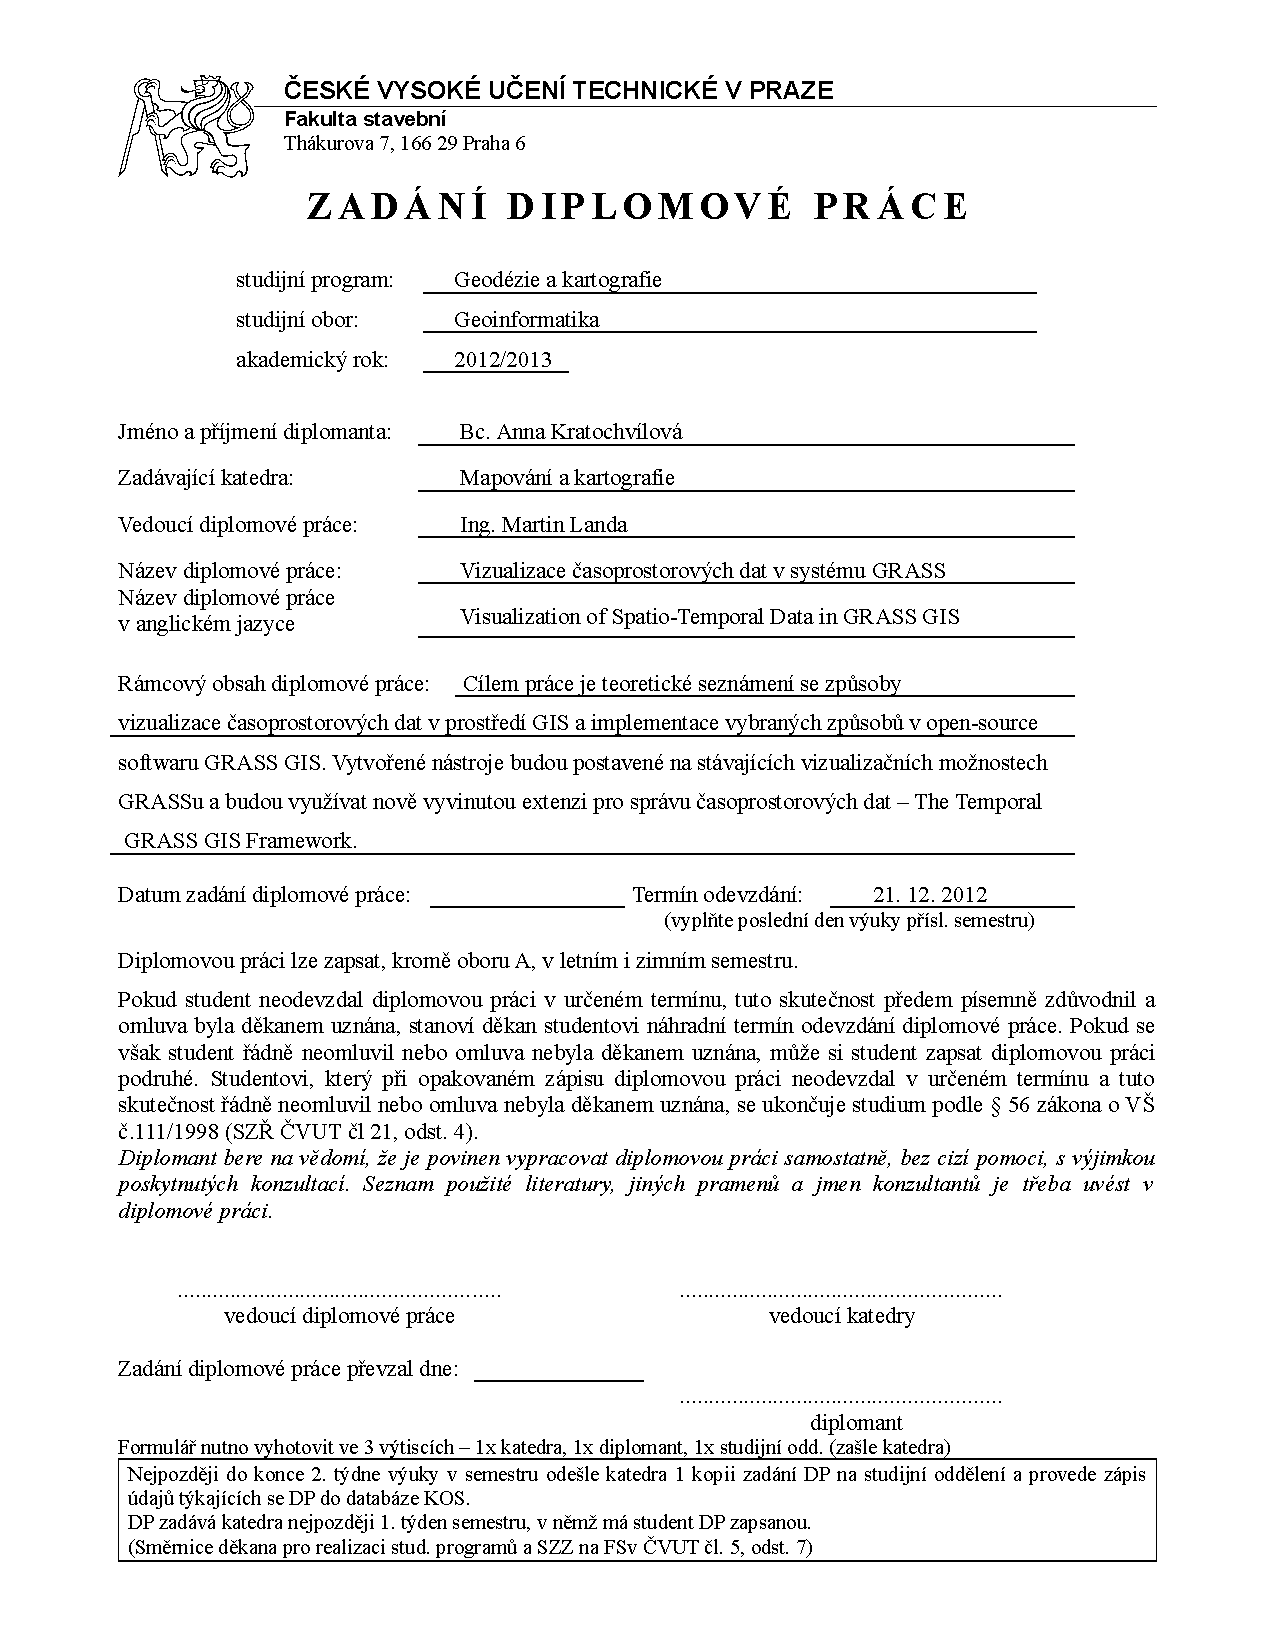
\includepdf[picturecommand={\put(0,200){\includeSubmission}}]{submission_empty}


% \begin{mtabstract}
The aim of this master thesis was to implement software tools for visualization
of spatio-temporal data in GRASS GIS. These tools make use of the recent addition
to GRASS 7, the GRASS GIS \tf which has been developed to manage, process and analyze
large scale, spatio-temporal environmental data.
Three new tools have been implemented, using the GUI toolkit wxPython, and incorporated into GRASS 7.
These applications include map animation, interactive comparison of two maps by ``swiping''
and visualization of temporal datasets' metadata.
The theoretical part of the thesis deals with spatio-temporal data in general, with special
focus on visualization approaches. List of currently available software
capable of handling spatio-temporal data is included.





\bigskip
\bigskip
\bigskip
\bigskip

\keyvalue{Key words}{GRASS, GIS, spatio-temporal data, visualization}

\end{mtabstract}

% \begin{mtabstract}[Abstrakt]

\selectlanguage{czech}
Cílem této diplomové práce je implementace nástrojů pro vizualizaci
časo\-pros\-toro\-vých dat v geografickém informačním systému GRASS.
Tyto nástroje využívají nedávno vyvinutého rozšíření GRASSu,
GRASS GIS Temporal Framework, který je určen pro správu, zpracování a analýzu
časoprostorových dat. Tři nové aplikace byly
vytvořeny pomocí grafické knihovny wxPython a začleněny do systému GRASS.
Mezi tyto aplikace patří nástroje pro animaci map, interaktivní porovnávání map
a vizualizaci metadat časoprostorových datasetů.
Teoretická část diplomové práce se zabývá časoprostorovými daty obecně,
a dále pak způsoby jejich vizualizace. Obsahuje také seznam současných softwarových
projektů, které jsou schopné zpracovávat časoprostorová data.


\bigskip
\bigskip
\bigskip
\bigskip


\keyvalue{Klíčová slova}{GRASS, GIS, časoprostorová data, vizualizace}
\selectlanguage{english}
\end{mtabstract}


% prohlaseni
\cleardoublepage
% \newcommand{\odsaditodzhora}{\hskip1pt\vfill}

\odsaditodzhora
\noindent Declaration of authorship

% I declare that I elaborated this diploma’s thesis on my own with the exploitation of the
% literature mentioned in the Bibliography section.
% I declare that I elaborated this master thesis on my own with
% the exploitation of the sources and literature mentioned in this work.

I declare that the work presented here is, to the best of my knowledge and belief,
original and the result of my own investigations, except as acknowledged.
Formulations and ideas taken from other sources are cited as such.

\begin{flushleft}
\begin{tabular}{cp{0.3\textwidth}c}
In Prague ................. 
&
&
..................................
\\
&&
(author's signature)
\end{tabular}

\end{flushleft}


% \chapter*{Acknowledgement}
\thispagestyle{empty}

First of all, I would like to thank my family for the encouragement and inspiration.

I would like to thank Martin Landa, my supervisor, for his support
and guidance during my work on this diploma thesis.

For providing insight into GRASS GIS \tf, as well as
for the opportunity to use it in my thesis, I would like to thank S\"{o}ren Gebbert, its author.

Also, I am grateful to Helena Mitášová for her ideas
which helped me to decide on the topic of my work.

I want to thank Robert Szczepanek for providing me with nice icons for the tools developed within my thesis.

Last, but not least, I would like to thank all the members of the GRASS Development Team and GRASS GIS users
who helped me by testing and suggesting improvements.


I acknowledge the E-OBS dataset from the EU-FP6 project ENSEMBLES\newline
(\url{http://ensembles-eu.metoffice.com)} and the data providers
in the ECA\&D project (\url{http://www.ecad.eu})



\cleardoublepage

\begin{center}

\newcommand{\logowidth}{3em}
\newcommand{\logospace}{\hspace{0.5em}}


\includegraphics[width=\logowidth]{./svg_images/cc}
\logospace

\includegraphics[width=\logowidth]{./svg_images/by}
\logospace

\includegraphics[width=\logowidth]{./svg_images/sa}

\bigskip

Visualization of Spatio-Temporal Data in GRASS GIS
by Anna Kratochvílová
is~licensed under a
Creative Commons Attribution-ShareAlike 3.0 Unported License.

\bigskip

\url{http://creativecommons.org/licenses/by-sa/3.0/}
\end{center}

% to choose license use:
% http://creativecommons.org/choose/

% download icons from
% http://creativecommons.org/about/downloads

% convert svg to pdf
% inkscape -z --export-pdf=file.pdf --export-area-drawing --export-dpi=300 file.svg


\tableofcontents
\cleardoublepage
\pagestyle{fancy}
\chapter{Introduction}
% http://upload.wikimedia.org/wikipedia/commons/2/29/Minard.png
Although the concept of time is intuitive, geographers, cartographers and other researchers have been
struggling with it from the early beginning of the existence of maps.
Unlike space dimension, time dimension has been ignored for a long time. For instance,
during 1817 - 1861, the establishment of the so called ``Stable''  cadastre by the Emperor Joseph II. 
in the whole Austrian Empire did not consider first the inevitable changes in the recorded data during the following years.
On the other hand, in 1869 (i.e.,\ almost at the same time)
a flow map on the subject of Napoleon's disastrous Russian campaign of 1812 was
published by a French civil engineer Charles Joseph Minard (see appendix \ref{appdx:minard}). This map is claimed to be
one of the best drawn historical graphics visualizing multiple variables where time is one of them.

In the past, research on spatial and temporal data representation and visualization
has mostly been conducted separately. However, during the last decades
effective integration of the spatial and temporal components was recognized as an vital assignment
since temporal information is necessary to better understand dynamic geographic processes
as well as the human-environment interaction. It can help us to answer questions such as:
How has the riverbed changed after the flood in February 24, 2005?
Which areas of agriculture land use have changed to urban land use during the last 10 years?
At what time of the day is the bus line overloaded and where?

Nowadays, the developers of geographic information systems (GIS) are aware that
processing of spatio-temporal data is what more and more users ask for.
Also the users of GRASS, an open source GIS, have now the possibility to manage,
process and analyze spatio-temporal data thanks to a new extension, the GRASS GIS \tf.
Since the \tf is not focused on data visualization in GRASS, the goal of this work
is to improve the spatio-temporal data visualization capabilities of GRASS GIS and in general,
to bring the \tf closer to the users. New visualization tools providing graphical user interface
are being developed; some of them make directly use of the \tf. These tools include tool
for animation, interactive comparing of maps and a support tool to visualize temporal dataset's metadata.

The work is organized as follows. In the next chapter \ref{chap:stdata}, I present issues connected with spatio-temporal data:
how we can represent it, visualize and explore, which software tools are currently available?
The following chapter \ref{chap:grass} is focused on GRASS GIS, its graphical user interface and, of course, the new \tf.
Chapter \ref{chap:results} finally introduces the newly developed tools and present their capabilities and implementation.







\chapter{Spatio-temporal data}
\label{chap:stdata}
The term \emph{spatial} data refers to data where each object has associated with it a location.
Naturally, \emph{spatio-temporal} data also include a temporal coordinate.
Spatial data have been collected, processed and visualized from the early history of mankind.
Conversely until today, the representation and visualization of spatio-temporal data
is problematic despite of great effort of researches all over the world.

This chapter summarizes main points about spatio-temporal data.
First a brief overview of the historical and current research efforts is presented.
Follows a description of several spatio-temporal data models and visualization techniques.
The last section mention some of the software tools for handling this kind of data.


\section{Efforts to integrate time with space}
Peuquet \cite{peuquet2001} provides an overview of the development of spatio-temporal data representation
and she reflects on the reasons of the still problematic situation.

One of the first areas which needed to handle temporal data were banking systems,
where storing temporal information about financial transactions is crucial.
This encouraged the DBMS (\emph{Database Management System}) to explore the possibilities of handling
temporal data. Simultaneously, a temporal database query language was being developed,
which resulted in TSQL2%
\footnote{There was an attempt to incorporate certain parts of this language
into new SQL standard SQL:1999, however the TSQL2 was later criticized
\cite{darwen2005}.} \cite{snodgrass1995}.
Recently, a new set of language extensions for temporal data support became a part of
SQL:2011 \cite{kulkarni2012}.

With the improvements in computer technologies and data capturing
(e.g.\ remotely sensed satellite data) researchers were able to empirically
study spatio-temporal patterns. These approaches were usually based on the
convenient \emph{snapshot} model (described in section \ref{sec:stModels}).

Since the attempts to represent time often lacked flexibility and suffered from other shortcomings,
the need for more theoretical view on space-time representation was recognized.
Peuquet \cite{peuquet2001} lists five areas as current research priorities:
    \begin{description}
      \item[The ontology of space and time]
      deals with the space and time on an abstract level. It tries to understand
      the concepts of linear vs.\ cyclic time, multiple times or different kinds of changes in time.
      
      \item[Development of efficient and robust space-time database models]
      is further discussed in section \ref{sec:stModels}.
      \item[Inexactness and scaling issues] refers to artificial discretization
      of continuous phenomena and imprecision in defining both spatial and temporal boundaries.
      \item[Graphical user interfaces]
      present the data so that the user can explore it conveniently and obtain it in the form he or she requires.
      \item[Indexing techniques for space-time databases] deals with optimized
      querying spatio-temporal data stored in a database.
     \end{description}

Since these issues have not been completely solved until today we can expect that research efforts
in this field will continue.
%%%%%%%%%%%%%%% ST models %%%%%%%%%%%%%%%%%%%%%%%%%%%%%%%%%%%%%%%%%%%%%%%%%%%%%

\section{Spatio-temporal data models}
\label{sec:stModels}
The capabilities of any information system depend on the design of its data models.
Spatio-temporal data modeling involves defining object data types,
relations and operations, and ensuring database integrity \cite{pelekis2004}.
Apart from that, a data model should take into account possible spatio-temporal queries and performed analyzes.

We have succeeded in modeling of spatial information;
current geographic information systems use raster, vector model or the combination of both.
Nonetheless, to model temporal information together with spatial information
has proved to be more complicated \cite{peuquet2001}.

In the following paragraphs, several spatio-temporal data models are described.
There is quite a large number of spatio-temporal data models (\cite{pelekis2004} identifies 11 distinct models), however
I decided to present only certain models which are frequently discussed in related literature.
The brief description should give an idea of spatio-temporal modeling
and it shows how spatio-temporal models vary.

\subsubsection{The snapshot model}
One of the simplest field-based spatio-temporal data models is the snapshot model.
This representation consists of a sequence of layers,
where each layer shows a state recorded at a certain point in time (see figure \ref{fig:snapshot_model}).
Hence, this model can be perceived as a 3D or 4D space-time cube \cite{peuquet2001}, for explanation of space-time cube refer to section \ref{sec:stcube}.

\begin{figure}[h!]
  \centering
  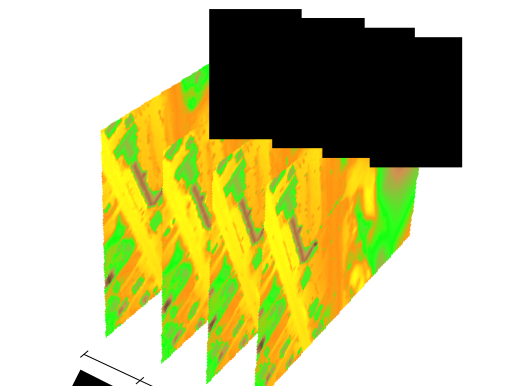
\includegraphics[width=0.6\textwidth]{./svg_images/snapshot_model.pdf}
  \caption{An illustration of snap-shot model}
  \label{fig:snapshot_model}
\end{figure}


The main drawback is the redundancy of data when there is little change between two successive states.
Also, it is not convenient to describe changes in space through time because the model captures only states.
Due to missing temporal structure, it is difficult to enforce integrity rules
and resolve all possible types of queries \cite{pelekis2004}.
It can be even compared to spaghetti model, term related to vector topology.
On the other hand, the advantage of this model is its simplicity;
it's implementation and usage is quite straightforward and intuitive.
In addition, it can be easily used to extend existent layer-based GIS.

To alleviate the problem of storing redundant data, an alternative approach,
\emph{Base state with Amendments} was suggested \cite{langran1988}.
This approach models changes instead of states.
The state can be retrieved by amending changes to the main state.
In order to improve the efficiency of retrieving a distant state,
various approaches have been suggested \cite{wang2012},
differing in the choice of base state or states and in the number and distribution of difference files.

\subsubsection{The space-time composite data model}
This model was suggested by Langran \cite{langran1988}. It assumes vector data representation.
The base map in this model is gradually fragmented as the changes occur.
Each fragment has its own attribute history represented by an ordered list of records.
To obtain a state at a point in time, all fragments are retrieved and common spatial boundaries are dissolved.
This model is conceptually straightforward, however the updating process may be more time consuming \cite{pelekis2004}
comparing to other models.
% The fragmentation requires to change identifiers each time when an old fragment is split into two new parts

\subsubsection{Event-oriented models}
According to \cite[p.~56]{temporalGlossary}, event ``\emph{is an instantaneous fact, i.e., something occurring at an instant}''.
The models mentioned above cannot clearly represent events.
In order to overcome this problem, events can be represented explicitly.
Several event-based models have been suggested by \cite{claramunt1995managing}, \cite{peuquet1995}, \cite{chen1998event}.

We can explain the basic concept of event-oriented models by describing
the raster-based approach implemented%
\footnote{The actual implementation used GRASS GIS for storing base map \cite{peuquet1995}.}
by Peuquet and Duan, called
\emph{Event-based Spatio Temporal Data Model} (ESTDM)  \cite{peuquet1995}.
This model stores changes associated with each time instance in an event list.
Every event from this list points to a list of event components,
which describe where changes occur (using efficient data structures).
Events are connected; every event has a pointer to the previous and the following event.
Similarly to the concept of amendments, there is also a base map, showing an initial snapshot.
ESTDM assumes that each event list and associated changes relate to a single thematic domain.

\subsubsection{Object-oriented models}
As object-oriented design showed promising results in the field of programming,
there were efforts to apply its features, such as classes and instances, attributes and methods,
inheritance and polymorphism, in spatio-temporal data model.

An object-oriented approach was for the first time applied by Worboys \cite{worboys1994unified}.
He suggested a unified spatio-temporal object (\emph{ST-complex}) which combines spatial component
with bitemporal component (event and database time). ST-complex is a collection of \emph{ST-simplexes}
where the spatial component represents a point, a straight line segment or a triangular area.
Operations like union, difference, boundary or spatial and temporal projection are defined for the ST-object.

Object-oriented models seem to have more advantages and less drawbacks comparing to other models.
Pelekis \cite[p.~27]{pelekis2004} claims that it can ``\emph{support  all types of data handling,
in terms of measurement, topological relationships and operations}''.

\subsubsection{The three domains model}
The three domains model was described by Yuan \cite{yuan1994wildfire}
and it was originally applied for wildfire modeling.
As the name suggests, the model has three domains, semantics, time, and space, which are interlinked.
In case of wildfire modeling, semantic domain can contain names of fire events, types or fire intensity.
The time domain describes the existence of semantic and spatial objects
(like geometrical primitives, cells and volumes).
Each domain can be handled separately in terms of database management system.
Thanks to the splitting of the spatio-temporal information,
this model is flexible enough to support wide range of spatio-temporal queries \cite{pelekis2004}.
The interesting aspect is that both splitting (the case of the three domains model)
and unifying (the case of the object-oriented model) can lead to good results.

%%%%%%%%%%%%%%% Visualization %%%%%%%%%%%%%%%%%%%%%%%%%%%%%%%%%%%%%%%%%%%%%%%%%%

\section{Visualization}
\label{sec:visualization}
Visualizing the world (through geospatial data) has been a cartographic interest for many centuries.
Current advanced software and hardware enable us to visualize geospatial data in many different ways,
however, existing visualization and exploratory techniques often do not suffice, especially in the temporal domain.

Visualization of spatio-temporal data is closely related to the term \emph{temporal map}.
Kraak and MacEachren \cite{kraak1994visualization} define temporal maps as
``\emph{a representation or abstraction of changes in geographical reality:
a tool (that is visual, digital or tactile) for presenting geographical information
whose locational and/or attribute components change over time}''.
They distinguish three categories of maps:
    \begin{description}
        \item[A single static map] represents an event by means of graphic sign system\,---\,from complex point symbols,
            temporal glyphs, to generalized trend-surface or flow-linkage maps depicting movement \cite{monmonier1990strategies}.

        \item[A strip map] represents an event by ordering `state' maps chronologically (as in `comic strip' style).
            Each map shows the state of the geographical reality at a unique time instance.
            The number of maps is rather limited because it is not possible to display long series of images
            due to lack of space (on paper or screen). Also, it would be too difficult to follow all these images.

        \item[Animated maps] represent an event by a quick chronological sequence of static maps.
            A typical example of animated map is shown during the weather forecast on television,
            where it depicts changing atmosphere's conditions.
            Fly-through animations are not considered to be temporal maps
            as long as there is no change in the spatial component (i.e.\ landscape).
    \end{description}

MacEachren \cite{maceachren1997exploratory} suggests a concept of visualization
where map usage is treated as a cube;
the axes represent the user of map (private vs.\ public),
objectives of use (revealing unknowns vs.\ presenting knowns)
and degree of interactivity (high vs.\ low).
One of the corners (private users, revealing unknowns and high interactivity)
represents \emph{visualization} and the opposite one \emph{communication}.
All maps involve both visualization (exploratory analysis leading to revealing new information)
and communication (delivery of desired information to map user),
however they differ in which component they underline.
Both components are important; first the researcher need to analyze the data
and then he explains his findings to the public.
In the following paragraphs I will focus mostly on the exploratory use of visualization tools.

In \cite{andrienko2003exploratory}, Andrienko et al.\ provides a review
of general exploratory techniques used for analysis of spatio-temporal data.
They based the task typology on work
%of Bertin \cite{bertin1983semiology}
of Peuquet \cite{peuquet1994s}.
She distinguished three view components in spatio-temporal data:
\emph{where} (space), \emph{when} (time) and \emph{what} (object).
This leads to three basic kinds of questions:
\begin{description}
    \item[when + where $\rightarrow$ what:]
        Describe the objects or set of objects (what) that are present
        at a given location or set of locations (where)
        at a given time or set of time (when).

    \item [when + what $\rightarrow$ where:]
        Describe the location or set of locations (where) occupied
        by a given object or set of objects (what) at
        a given time or set of times (when).

    \item [where + what $\rightarrow$ when:]
        Describe the times or set of times (when) that a given
        object or set of objects (what) occupied a
        given location or set of locations (where).
 \end{description}

The techniques described below differ in the fact how well they can answer these questions.
The classification of the techniques regarding this aspect is presented in \cite{andrienko2003exploratory}.
Here we focus on the general characteristics.
% For the purpose of their work, Andrienko et al. simplified this classification into two cases:
%     \begin{description}
%         \item[when $\rightarrow$ where + what:]
%             Time is given and other information (location, characteristics) has to be found out.
%         \item[where + what $\rightarrow$ when:]
%             With other types of information, time has to be discovered.
% 
%      \end{description}
%  

\subsection{Exploratory techniques}
\label{sec:exploratoryTechniques}
Unlike paper maps, computer-based visualization tools offer many important features
such as interactivity and dynamics which are necessary for most exploratory techniques
like map querying or animation.

\subsubsection{Querying}
A query consists of two main parts\,---\,target and constraints \cite{andrienko2003exploratory}.
For example, we can ask where (target) a particular object was located at a given time instance (constraint).
A query can be specified by the user either by a machine-readable language (typically Structured Query Language)
or via graphical user interface (possibly using Visual Query Languages \cite{catarci1997visual})
which is usually more convenient for end-users who then tend to perform tasks faster.
An example of dynamic query tools which constrain the query can be found
in \cite{ahlberg1992dynamic} and \cite{hochheiser2004dynamic}.
However, dynamic query tools usually do not allow to build a more complicated query;
for example, when logical \emph{OR} and \emph{AND} are combined.

% Often, the query constraints are specified by a mouse cursor pointing at a location on map.

In case of temporal queries, specific graphical user interface
might be needed. Figure \ref{fig:cyclical_time} shows a temporal query tool
which enables to select arbitrary combinations of years, month, days and hours.


\begin{figure}[h!]
  \centering
  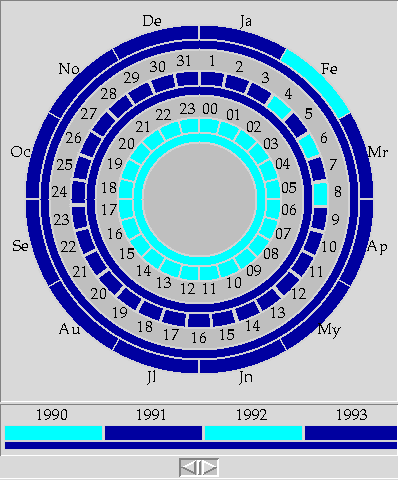
\includegraphics[width=0.5\textwidth]{./images/cyclical_time.png}
  \caption[Widget for temporal queries from system TEMPEST]
        {Widget for temporal queries from system TEMPEST (Source:
      \url{http://w ww.geovista.psu.edu/products/demos/edsall/Tclets072799/cyclicaltime.htm})}
  \label{fig:cyclical_time}
\end{figure}



\subsubsection{Map iteration}
\label{sec:mapIteration}
Map iteration corresponds to the term ``strip maps'' mentioned before.
Temporal information is presented as a juxtaposition of several maps.
Each map represents one state of a phenomenon at an time instance.
This technique can be used with both conventional maps and maps on computer screens.
Also, it is applicable for all type of spatio-temporal data.

The technique of map iteration is suitable
for detection of a change and for finding the moment when the change occurred
by shifting the focus from one map to the other.

This task can be made even easier by overlaying one map over the other providing that the upper map is semitransparent.
This makes the changes more visible.
However, from my own experience, such a tool should allow the user to change the transparency level dynamically
because certain changes might be revealed easier at a different level of transparency.
Similar approach is the fading technique.
One map gradually disappears while the next map emerges from beneath of it.

Another variation on the topic which is not mentioned in \cite{andrienko2003exploratory}
is `swipe' technique.
It allows the user to interactively compare two layers (typically raster)
of the same area by revealing different parts of the maps (see for example figure \ref{fig:swipe}).


\begin{figure}[h!]
  \centering
  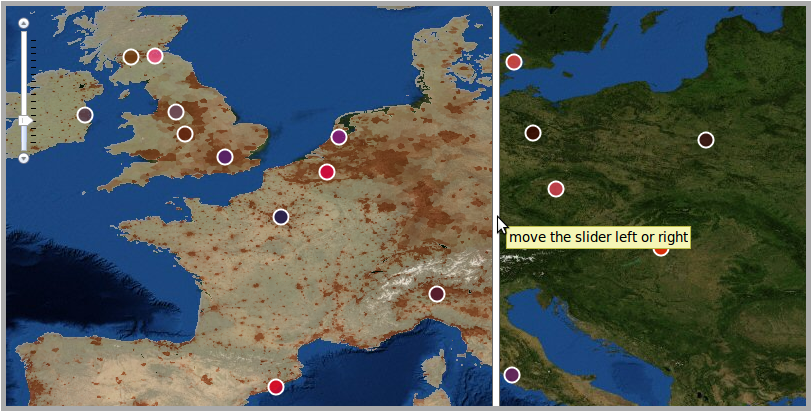
\includegraphics[width=0.8\textwidth]{./images/swipe_example.png}
  \caption[Example of `swipe' technique]
  {Example of `swipe' technique. Source: \url{http://sathyaprasad.appspot.com/swipe.html}}
  \label{fig:swipe}
\end{figure}


\subsubsection{Map animation}
\label{sec:mapAnimation}
Unlike map iteration, map animation is a technique which is applicable for computer screens only.
Nonetheless, there is only a few steps from map iteration to map animation.
Instead of displaying a series of static maps, there is a single map but its content changes.
The changes representing an event are inferred from real movement on the map.
Animation consists of frames\,---\,single images (maps).

\paragraph{Application}
Animations can be useful to reveal trends, processes and subtle spatio-temporal patterns
that are not evident in static representation. Dorling and Openshaw \cite{dorling1993using}
demonstrated a power of animated maps to stimulate knowledge;
they investigated childhood leukemia rates in northern England during twenty years.
Thanks to the animation the previously unrecognized hot-spots (localized both in space and time) emerged
as well as the oscillation between the rise and fall of the incidence of
cases in Newcastle and Manchester. Since time component was not considered in previous studies,
they failed to reveal these patterns.

Animation can be used to visualize routes of moving objects \cite{andrienko2003exploratory}.
Unlike static representations, animation can reveal details about speed, acceleration and interaction
of the individual objects. Consider the case when the trajectories of two objects cross each other.
Without animation we are not able to decide if the objects really met or
if they just arrived at the same place in a different moment.
There are three alternative approaches to visualize object movement by animation \cite{andrienko2003exploratory}:
    \begin{description}
        \item[Snapshot in time] The simplest approach is based on displaying the objects
        at their location at the given time instance. This method is usually not convenient for more than one object.
        \item[Movement history] Beside the objects, also their trajectories are displayed from the starting point.
        When the animation ends, complete trajectories are shown. This approach prevents the user from loosing track,
        however in case of more complicated trajectories, the situation might become too complex.
        \item[Time window] Similarly to the previous approach, trajectories are displayed.
        However only a part of the trajectories corresponding to the last few time units are visible,
        like the white trails leaved behind by a plane.
        This method solves the drawback of the `movement history' method.
        An example of such approach is in figure \ref{fig:shark}.
    \end{description}



\begin{figure}[ht]
\centering
    \begin{subfigure}[ht]{0.3\textwidth}
    \centering
        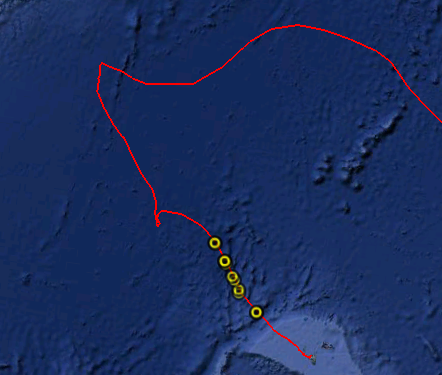
\includegraphics[width=\textwidth]{./images/shark_move_1.png}
    \label{fig:shark1}
%     \caption{Shark}
    \end{subfigure}
    \begin{subfigure}[ht]{0.3\textwidth}
    \centering
        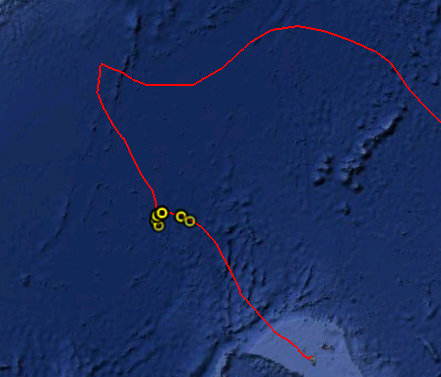
\includegraphics[width=\textwidth]{./images/shark_move_2.png}
    \label{fig:shark2}
%     \caption{Shark}
    \end{subfigure}
    \begin{subfigure}[ht]{0.3\textwidth}
    \centering
        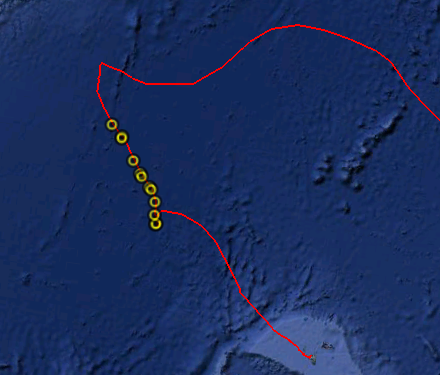
\includegraphics[width=\textwidth]{./images/shark_move_3.png}
    \label{fig:shark3}
    \end{subfigure}
\caption[Trajectory of a whale shark visualized in Google Earth]
{Trajectory of a whale shark visualized in Google Earth
(data source: German European School Singapore).
Red line symbolizes the trajectory and the yellow circles represents measurements of shark's position.
Each picture shows the measurements from a different time interval.}
\label{fig:shark}
\end{figure}

%%%%%%%%%%%%%%%%%%%%%%%%%%%%%%%%%%%%%%%%%
\paragraph{Dynamic visualization variables}
In \cite{dibiase1992animation}, DiBiase et al.\ introduced three dynamic visualization variables of animation:
\emph{duration}, \emph{rate of change}, \emph{order}.
Three more variables were added by MacEachren \cite{maceachren2004maps}:
\emph{frequency}, \emph{display time} and \emph{synchronization}.
According to Kraak \cite{kraak2000visualisation}, duration and order are the most important
dynamic variables. Duration is the time interval during which no change on the display occurs.
Order, the succession of individual frames, together with duration can be used to
\emph{``express an animation's narrative character''}\cite[p.~31]{kraak2000visualisation}.
Frequency is the number of identifiable states per unit of display time.
Despite the fact that frequency is the dual of duration,
\emph{``it is worth treating as a separate dynamic variable because \ldots
humans react to frequency as if it were an independent variable''} \cite{kraak1994visualization}.
Display time, also called \emph{moment of display}, refers to the time when some display change is initiated.
According to Blok  \cite{blok2005dynamic}, synchronization and rate of change are not dynamic variables
but effects of interaction with other dynamic variables.

The last mentioned variable, synchronization, refers to the possibility to run two or more
animations simultaneously. This might reveal synchronization of patterns between (possibly related) phenomena.
Also it may be useful to experiment with different starting moments of animations.
This allows to explore cause-effect relationships between phenomena, for example
the delayed effect of precipitation on vegetation growth.
However, it is unclear whether an analyst is able to effectively watch two or more simultaneous
juxtaposed animations \cite{andrienko2003exploratory}. More research need to be conducted.
Using the eye-tracking technology seems to be one possible approach
(see for example study \cite{opach2011evaluating}).

%%%%%%%%%%%%%%%%%%%%%%%%%%%%%%%%%%%%%
\paragraph{Temporal legend}
In \cite{kraak1997cartographic}, Kraak et al.\ deal with temporal legend for animations.
Temporal legend is the part of the interface which does not only help to understand and interpret
the phenomenon but it can also serve as navigation tool to control dynamically the animation.
In order to explore spatio-temporal data, animation should offer functionality like replaying, pausing
and going to a particular frame.
Temporal legend can differ according to the type of displayed data.
For example, certain kinds of data, like hourly measured temperature, have naturally perceived periodic pattern.
For those data, clock-like legend might be more suitable.
However it describes only the temporal location within one cycle.

On the other hand, for several kinds of data linear time representation is more natural (e.g.\ erosion process)
and for this case a slide bar, where the marker shows the current temporal location, would be a better choice.
Both types of temporal legends could be accompanied by numerical legend (e.g.\ 23:14,  March 2012, \ldots)
as suggested by Kraak \cite{kraak1997cartographic}.
However, a study showed that the choice among these three types of legend has no significant effect on
the performance, response times or correctness of results \cite{edsall1997assessing}.

Another types of temporal legend for animation can try to avoid the distracting the user.
Sound legend can signalize either the date and time or the animation frequency (by ticking).
Another approach applicable only for certain data is based on changing the brightness of the screen
to induce an illusion of day and night.

% about animation in public - presentation, web, education
% TODO: add ref from Helena  - ROLE OF DYNAMIC CARTOGRAPHY IN SIMULATIONS OF LANDSCAPE PROCESSES BASED ON MULTI-VARIATE FIELDS
% skagit.meas.ncsu.edu/~helena/gmslab/papers/listsj.html

\subsubsection{Space-time cube}
\label{sec:stcube}
The space-time cube is basically a 3D plot in which the spatial component (e.g.\ a geographic map)
is plotted in the $xy$\nobreakdash-plane and the temporal domain is represented
on the vertical $z$-axis (see figure \ref{fig:stcube_cut}).

\begin{figure}[h!]
  \centering
  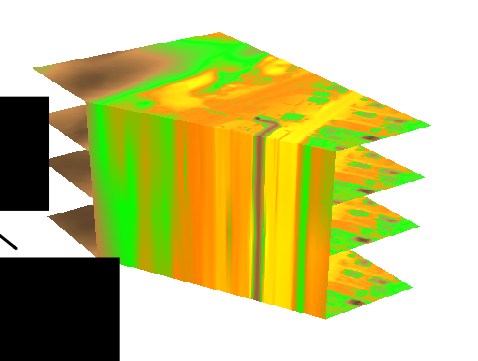
\includegraphics[width=0.6\textwidth]{./svg_images/snapshot_cut.pdf}
  \caption{An illustration of space-time cube}
  \label{fig:stcube_cut}
\end{figure}

This new view on time as an additional spatial dimension was introduced in 1970 by Hägerstrand \cite{hagerstrand1970}.
He suggested a three-dimensional diagram, the space-time cube, to study the space-time behavior of human individuals.
In those days, creating graphics was limited to manual methods.
Therefore creating an alternative view on the cube, which is essential for this visualization technique,
required an arduous drawing process. Today, thanks to modern computer technologies, much better opportunities
for visualization are provided. As a result, researchers bring back this concept and
investigate it in order to use it as a new exploratory tool.

Space-time cube is a concept which is applicable for various analyses and type of data.
We can find several different employment of space-time cube in literature.
The usages differ in the purpose of analysis which is then closely related
to the type of analyzed data (vector lines, points, voxel data).

\paragraph{Space-time path}
The original Hägerstrand's concept was concerned with movement of objects (people).
During day each person follows a trajectory through space and time called
\emph{space-time path}. Figure \ref{fig:st-path} shows a simplified example
of persons movements during a working day. The locations where people stay,
called \emph{stations} (e.g.\ at home, at work), are represented by a vertical direction of the path.
However in a larger scale, we could observe movement at these stations
(people moving inside buildings). The time when people meet at a station is called \emph{activity bundle}.

Figure \ref{fig:st-prism} schematically shows a \emph{space-time prism}
which indicates the locations that can be reached in a particular time interval
(starting and returning to the same place). In reality, it is not circular because
not all places are accessible.




\begin{figure}[ht]
\centering
    \begin{subfigure}[ht]{0.49\textwidth}
    \centering
        \includegraphics[width=\textwidth]{./svg_images/space-time-path.pdf}
    \caption{Space-time path}
    \label{fig:st-path}
    \end{subfigure}
    \begin{subfigure}[ht]{0.49\textwidth}
    \centering
        \includegraphics[width=\textwidth]{./svg_images/space-time-prism.pdf}
    \caption{Space-time prism}
    \label{fig:st-prism}
    \end{subfigure}
\caption{Space time path}
\label{fig:st-path-prism}
\end{figure}


Space-time paths are naturally applied to movement data, such as public transport data \cite{transport2005visualisation}.
Apart from that, space-time paths are often used to analyze sociological aspects
as for example in the study focused on non-employment activities with regard to gender \cite{kwan1999gender}.
In \cite{moore2003time}, this technique was used in sport to analyze rugby matches.
Additionally, Kraak \cite{kraak2005visualization} suggests to use it for real-time monitoring which is possible thanks to
the boom of GNSS (Global Navigation Satellite System) technologies.
Another discipline which may benefit from the space-time paths approach is archeology.
Kraak \cite{kraak2005visualization} provides an example of space-time paths representing
archeology excavations where the stations indicate the duration of the existence of settlements.
Another study concentrated on the interaction of cultures using a combination of the space-time cube approach
with graph theory \cite{huisman2008development}.



% understand An Evaluation of Space Time Cube Representation of Spatiotemporal Patterns

% GNSS influenced makes collecting


\paragraph{Event data}
Space-time cube concept is suitable not only to represent moving objects
but it can be successfully applied to events, too.
Gatalsky et al.\ \cite{gatalsky2004interactive}
focused on the detection of spatio-temporal patterns in event occurrences.
In their work, events (earthquakes) are represented as circles placed vertically according to their occurrence.
Size and color of each circle reflect the thematic characteristics of the event.
The space-time cube is dynamically linked to a map display so that it is possible to highlight corresponding events.
% By using this method, they were able to find grouping

\paragraph{Voxel data}
\label{voxelHelena}
Another potentially large field of study is the application of space-time cube concept for voxel data.
Mitasova et al.\ \cite{mitasova2011landscape} presents a multidimensional framework for characterization
of land surface dynamics using time series of elevation data (LiDAR point cloud).
Space-time cube, as one part of this framework,
creates a voxel representation of elevation evolution with time as a third dimension.
The evolution of contour-based features (shorelines) is studied
by visualization of multiple isosurfaces extracted from the voxel model%
%(\ref{fig:})
.
In this context, an isosurface represents a contour of given $z$-coordinate (height)
stretched in the vertical time dimension.
% TODO: add images of voxel schema, isosurfaces http://www.sciencedirect.com/science/article/pii/S0169555X11002935

\paragraph{3D glyphs}
Space-time cube approach is also used to visualize distributions of
geospatial time-varying data through a pictorial representation \cite{tominski20053d,thakur20103d}.
A base map is typically divided into regions or administrative districts.
Above each of these parts, a 3D icon or glyph is drawn.
In \cite{thakur20103d}, the glyph is represented by a set of disks stacked along the vertical temporal axis,
one for each time step. The size of the disk is scaled according to maximum disk size.
Additionally, color is used to encode data values and although it is redundant
(the information is already in the disk size), it can help to detect outliers.
This visualization technique helps an analyst to quickly explore multiple time-varying
quantities on a map and extract useful information.



\paragraph{}
As illustrated in the paragraphs above, space time cube approach
can be applied in various domains. The increased interest in this technique seems
to be caused by rapid improvements in computer technologies as well as by simplification and speeding
data collection process by GNSS technologies and remote sensing.

Although space-time cube is a useful exploratory tool it might not always be helpful
for novice users because of problems with its interpretation. A study \cite{kristensson2009evaluation}
showed that novice users benefit from the space-time cube representation only when they are asked to analyze
complex spatio-temporal patterns. In case of simpler tasks, using the space-time cube representation
led to higher error rate comparing with using a 2D representation.






\section{Existing software}
The list of GIS software on Wikipedia \cite{wiki:gislist}
shows us that there exist many geographic information systems,
both open-source and proprietary.
However, the number of GIS or other related applications which can handle
spatio-temporal data is much smaller.
This is not surprising considering the fact that GIS development started
in the 1960s \cite{coppock1991history} while the initial efforts to model spatio-temporal
data appeared in the 1980s and later \cite{peuquet2001}.

In \cite{andrienko2003exploratory} from 2003, a partial review of existing systems is provided.
However, it was not meant to be complete. Moreover, it contains mainly research prototypes,
which are often very specialized and serve for academic purposes only, although their implementations
and features can be innovative and useful.
Since 2003, some of these projects have been renamed,
moved to newer websites or they just disappeared or they are not maintained anymore.
On the other hand, new tools have been developed.
For example, we can witness the expansion of web-based applications in the recent years.
It seems that visualizing time dimension becomes `modern'.

The following list of software able to process and or visualize spatio-temporal data is not comprehensive.
It includes only the main systems with large user base.
Often these systems are not intended primarily for temporal data,
but they started to provide this functionality because of the users' needs
and also to keep up with new trends in GIS.


\subsection{Free and open-source software}
\subsubsection{GRASS GIS: Temporal Framework}
A new GRASS GIS Temporal Framework extends significantly the capabilities of GRASS GIS
to process spatio-temporal data. For more information see section \ref{sec:GRASSTF}.

\subsubsection{QGIS: Time Manager}
QGIS\footnote{\url{http://www.qgis.org/}} is a rapidly developing cross-platform
geographic information system. Time Manager\footnote{\url{https://github.com/anitagraser/TimeManager/}}
is a plugin for animating maps, currently multiple vector layers are supported.
It allows basic animation functionality (to control the animation flow) and
users can specify offset for each layer separately.

QGIS and Time Manager are under the GNU General Public License%
\footnote{http://www.gnu.org/licenses/gpl.html}.

\subsubsection{R: spacetime package}
R software is a powerful software environment for statistical computing and graphics.
A new package \emph{spacetime} has been added recently \cite{PebesmaR} to support spatio-temporal data.
This package is built upon \emph{sp} package for spatial data and
\emph{xts} package for time series data.
The package introduces four space-time layouts (full grid, sparse grid, irregular, trajectory)
which represent the basis of the implemented classes.
The package handles both raster and vector types of data.
It allows to select, manipulate, visualize data and use any other needed functionality
available from other packages. However it's not meant as a database:
the data are imported first, then processed and the output is saved.

R software is under the GNU General Public License.

\subsubsection{GeoVISTA software}
GeoVISTA Center on Penn State University is focused on the development of applications
and toolkits that allow scientists analyze different kinds of geospatial data.
Several applications are able to handle spatio-temporal data.

\paragraph{ESTAT}
ESTAT: The Exploratory Spatio-Temporal Analysis Toolkit%
\footnote{\url{http://www.geovista.psu.edu/ESTAT/}},
is developed by the GeoVISTA
center on Pennsylvania State's University. It is written in Java and designed to support exploratory
geographic visualization. It presents spatio-temporal multivariate data
in a dynamically-linked environment; it includes scatterplot, bivariate choropleth map%
\footnote{Choropleth map is a thematic map in which areas are colored
(or patterned) proportionally to the measurement of the displayed statistical variable.
Bivariate choropleth map is explained in \cite{leonowicz2006two}.},
parallel coordinate plot and time series graph.
ESTAT is used for epidemiology research but it can handle other types of data as well.

ESTAT is an open-source software built upon GeoVISTA Studio development environment
licensed under the GNU Lesser General Public License%
\footnote{\url{http://www.gnu.org/copyleft/lesser.html}}.

\paragraph{STempo}
STempo\footnote{\url{http://www.geovista.psu.edu/stempo/}} is a software prototype aimed at
understanding of geolocated events and their relationships.
It enables to derive patterns at multiple spatial and temporal scales by innovative statistical procedures,
with integrated interactive visualization.
STempo consists of different views including a map, a time line,
a concept-based view represented by a tag-cloud and a table presenting data.
These views can be used for selecting and filtering event data.

STempo is an open-source software built upon Visual Inquiry Toolkit and GeoViz Toolkit
licensed under the GNU Lesser General Public License.

\subsubsection{PCRaster}
PCRaster\footnote{\url{http://pcraster.geo.uu.nl/}}
is a collection of software tools and libraries focused on the spatio-temporal
environmental modeling (hydrology, ecology, etc.). It processes raster maps only.
PCRaster allows to develop their own simulation models using scripting languages PCRcalc and Python.
Interactive visualization component is called Aguila
which replaced the two former components focused on visualization of raster maps
and time series separately.

PCRaster is developed mainly for research and educational purposes by
Faculty of Geosciences at Utrecht University in the Netherlands.
PCRaster software is partly distributed under GNU General Public License (PCRaster Open Source Tools),
and partly under a closed source license.

\subsubsection{TerraLib and TerraView}
TerraLib\footnote{\url{http://www.terralib.org/}} is an open-source GIS software library.
It supports large-scale applications using socio-economic
and environmental data \cite{camara2008terralib}.
% TerraLib extends object-relational DBMS
% technology to support spatio-temporal models, spatial analysis, spatial data
% mining and image databases.
TerraLib supports the development of geographical applications
using spatial databases, and stores data in different database management systems (DBMS)
including MySQL and PostgreSQL. Its vector data model is compliant with Open Geospatial
Consortium (OGC) standards. It handles different spatio-temporal data types (events,
moving objects, modifiable objects) and allows spatial, temporal and
attribute queries on the database. Moreover, TerraLib provides a  direct link with the
R programming language for statistical analysis through aRT package.

TerraView\footnote{\url{http://www.dpi.inpe.br/terraview_eng/index.php}}
is an application built on the TerraLib library
which provides functions for data conversion, display, exploratory spatial data
analysis and spatial and non-spatial queries.

TerraLib and TerraView are being developed by a development team based in Brazil
under the GNU Lesser General Public License and GNU General Public License, respectively.


\subsubsection{Web-based software}
Since many GIS-based applications are currently moving from desktops to web, it is not surprising that
new web-based libraries and programs focused on  spatio-temporal data visualization appear.
Web applications are mostly concerned with the `communication' corner in terms of the cube analogy
(explained in section \ref{sec:visualization})\,---\,they try to present the information
in an interesting and attractive way. This is connected with the fact that GUI for web application
tends to be  far more flexible and the traditional widgets are enriched by new innovative features.
This can help to improve the visualization of the spatio-temporal data.

\paragraph{i2maps} i2maps\footnote{\url{http://ncg.nuim.ie/i2maps/docs/}} is a software environment for geocomputation.
It consists of two libraries, one written in Javascript, and the other in Python.
The Javascript library is used for building the interactive user interface, and is built on top of OpenLayers.
The Python library consists of a server-based interface for linking data sources
and spatio-temporal analysis modules to the Javascript library, and is built around the GeoDjango framework.
i2maps provide libraries that make it easier to write software for collecting,
processing, modeling, visualization spatio-temporal data.

i2maps is distributed under an unspecified open-source license.

\paragraph{\emph{Time}Map} \emph{Time}Map TMJava is a mapping applet
which generates interactive maps. Applet can be embedded into web page
or it can be run standalone.
\emph{Time}Map claims to be the first web mapping applet which provides
generalized support for temporal maps, including time-filtering and animation.
TMJava can connect with databases which are being actively updated.

\emph{Time}Map is released under the GNU General Public License.

It is worth mentioning that there seems to be no activity on this project since 2008 according to
Ohloh\footnote{\url{http://www.ohloh.net/}} statistics.

\paragraph{timemap.js}
Timemap.js\footnote{\url{http://code.google.com/p/timemap/}}
is a Javascript library designed to help to use online maps,
including Google, OpenLayers, and Bing, with a SIMILE time line.
This time line widget comes from SIMILE Widgets which focus the development of data visualization web widgets.
The timemap.js library allows to load one or more datasets in different formats (JSON, KML, or GeoRSS)
onto both a map and a time line simultaneously.

Timemap.js is licensed under the MIT License\footnote{\url{http://opensource.org/licenses/mit-license.php}}.



\subsection{Proprietary software}
\subsubsection{ArcGIS: Tracking Analyst}
Tracking Analyst is an ArcGIS (ESRI) extension for spatio-temporal data focused on vector data \cite{arcgisHelp}.
It is designed for mapping of moving objects or objects with changing attributes.
Tracking Analyst include exploratory tools such as animations, time window approach based on symbology,
creating special charts and other sophisticated tools.
Further, it supports viewing data in 3D using ArcGlobe. 
ArcGIS itself provides data storage mechanism\,---\,the primary storage option is the geodatabase.

The price of a single use license (e.i., for a single desktop computer)
of Tracking Analyst is currently \$2,500%
\footnote{source: \url{http://www.esri.com/software/arcgis/extensions/trackinganalyst/pricing}}.
The price of ArcGIS itself (which is not publicly available) is not included.

\subsubsection{STEMgis}
STEMgis (Discovery Software) is a temporal GIS which provides the tools to manage, visualize
and analyze undergoing changes,
It can be used for environmental, coastal, marine, health, crime, sales and marketing,
agriculture and forestry applications.
It consists from three parts: STEMgis Manager (data management), 
STEMgis Viewer (multidimensional visualization and analysis),
STEMgis Publicist (data publication including a freely distributable version of STEMgis FreeView).
The full list of features, examples and animations can be found on the official home page of this software%
\footnote{\url{http://www.discoverysoftware.co.uk/STEMgis.htm}}.

STEMgis claims to be an affordable GIS: a commercial license for STEMgis is \pounds150,
while an academic license is \pounds100.

\subsubsection{GeoTime}
GeoTime 5\footnote{\url{http://www.geotime.com/}} (Oculus)
is data visualization and analysis software, specializing in
the display of events over time. GeoTime provides tools
for law enforcement analysts, including cell site analysis, mobile forensics data analysis
and crime series analysis. It visualize data by innovative 3D Time Viewer offering a sophisticated but 
easily understandable view on the data based on space-time path approach.
GeoTime enables to automatically detect spatio-temporal patterns like meetings, gaps, motion and connections.
Also it provides extensions to cooperate with ArcGIS and spreadsheet application Microsoft Excel.

The GeoTime Standalone Starter Pack is priced at \$3975\footnote{source:
\url{http://www.geotime.com/Buying-GeoTime.aspx}}.



\subsubsection{Google Earth}
Google Earth is a wide-spread software for visualization and exploring places all over the world
using a virtual globe.  It maps the Earth by the superimposition of images
 from satellite imagery and aerial photography which are keeping up-to-date.
Although Google Earth is a desktop application (also available on web and mobile phones) it needs
the Internet connection to download data and display it.

The native data format used to add custom data to Google Earth is the XML-based Keyhole Markup Language (KML).
By adding time stamps to features in the KML file, time component can be visualized. KML distinguishes
between time instances and time intervals. When time component in the data is detected,
a time slider is enabled automatically. An interesting feature, AbstractViews, enables to automatically
adjust the sunlight and historical imagery according to the time specified in the KML tags.

Google Earth offers a free version with limited functionality and usage.
Google Earth Pro version is licensed at \$399 per user per
year\footnote{source: \url{http://www.google.com/earth/explore/products/desktop.html}}.




\chapter{GRASS GIS}
\label{chap:grass}
\section{General overview}
GRASS  (Geographical Resources Analysis Support System)\footnote{\url{http://grass.osgeo.org}}
is a general purpose cross-platform open-source geographic information system (GIS)
with raster, vector and image processing capabilities \cite{neteler2011grass}.
It includes more than 350 modules for managing and analyzing geographical data.
GRASS was created in the early 1980s by the Construction Engineering Research Laboratory (CERL)
of the United States Army as a software management tool for military applications.
Nowadays it is one of the cutting-edge projects of the Open Source Geospatial Foundation
(OSGeo\footnote{\url{http://www.osgeo.org/}}, founded in 2006).
Quoting Neteler and Mitasova \cite[p.~3]{grassGisApproach}:

\begin{quote}
The key development in recent GRASS history was the adoption of GNU GPL
(General Public License, see http://www.gnu.org) in 1999.
With this, GRASS embraced the Open Source philosophy,
well known from the GNU/Linux development model, which stimulated its wide acceptance.
\end{quote}

% The adoption of the free software license changed the development process
% of GRASS GIS with contributions to the source code becoming decentralized.
The legal statements declared in the GPL are based on the ``four freedom'' paradigm \cite{stallman1985gnu}
and allow the user to use the software’s full range of capabilities, and to distribute, study and improve it.
The revision control system of GRASS GIS (namely subversion\footnote{\url{http://subversion.apache.org/}})
allowed different institutions and individuals to contribute to the code base
from different countries around the world.

The modular software design of GRASS facilitates the introduction of new functionality.
Moreover, its scripting capabilities enable automated processing of a large volume of data.
Since 2008, GRASS users and developers can make use of the Python programming language \cite{van1995python}
to introduce new features. Integration between GRASS and Python has been recently enhanced through a new,
more ``pythonic'' API \cite{pygrass} which provides easier, more natural and consistent scripting possibilities.

GRASS is a project which is actively developed and tested by users from different
countries using different platforms.
At this time a new stable version 6.4.3 is about to be released, however
the developers mainly focus on GRASS 7 which has already many improvements:
new raster, vector and image processing modules, speedup of the vector engine,
improved portability (MS Windows, Mac OS X), modern graphical user interface (GUI) and others.
Not only programmers are involved, also many translators contribute to this project
in order to make it accessible for users from non-English speaking countries.
Also users are involved in the process of development by testing and providing feedback.
Through the issue tracking system\footnote{\url{http://trac.osgeo.org/grass/}},
they can report any software bug or suggest an improvement.

% interoperability?

\section{GRASS GIS Graphical User Interface}
\label{sec:grasswxgui}
Originally, GRASS was controlled only through command line interface (CLI).
Later, a need for graphical user interface (GUI) appeared
which led to the first GUI prototype called \emph{TCLTKGRASS}
written in \emph{Tcl}\footnote{\url{http://www.tcl.tk}}
programming language using \emph{Tk} graphical toolkit.
However, during the 2000's the limitations of Tcl/Tk toolkit turned out to be
an obstacle for further development \cite{wxGUI2008}.
In 2006, it was decided to build a new GUI based on
\emph{wxPyton}\footnote{\url{http://www.wxpython.org}}\,---\, a Python wrapper
for cross-platform GUI toolkit \emph{wxWidgets}\footnote{\url{http://www.wxwidgets.org/}}.
Among other benefits, Python programming language is far more popular than Tcl
and it is also much easier to learn which enlarges the number of potential contributors.

The new graphical user interface, called wxGUI, has been developed since 2006.
It consists of three core components:
    \begin{enumerate}
      \item \emph{Layer Manager} allows users to launch different GRASS modules from menu,
      manage layers. Command-line prompt, command output window and python shell
      for scripting are integrated (figure \ref{fig:wxGUI1}).
      \item \emph{Map Display Window(s)} provides basic tools for zooming, panning, data querying,
      decorations (legend, north arrows, bar scale).
      During one session, multiple Map Displays can be opened (figure \ref{fig:wxGUI1}).
      \item \emph{module dialogs} are generated for each GRASS module from the XML interface description.
      This approach enables to create GUI for every module while respecting its particular parameters
      (figure \ref{fig:wxGUI2}).
    \end{enumerate}

\begin{figure}[ht!]
\centering
    \begin{subfigure}[ht]{\textwidth}
    \centering
        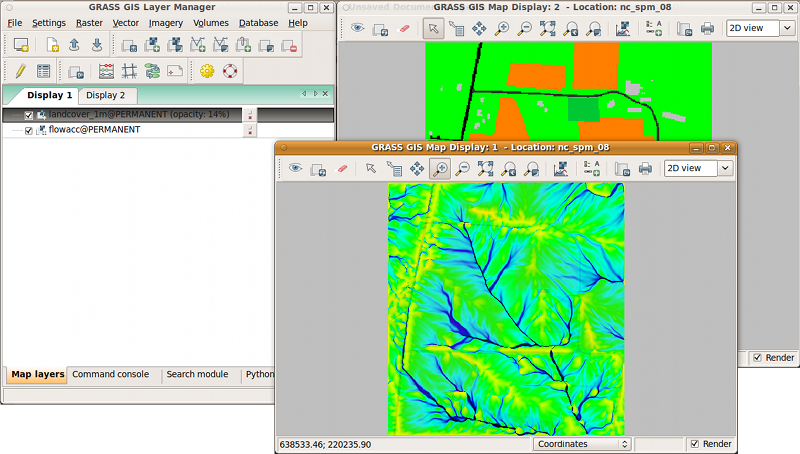
\includegraphics[width=\textwidth]{./images/wxGUI_1.png}
    \caption{Layer Manager and two Map Display Windows}
    \label{fig:wxGUI1}
    \end{subfigure}

\vspace{10pt}

    \begin{subfigure}[ht]{\textwidth}
    \centering
        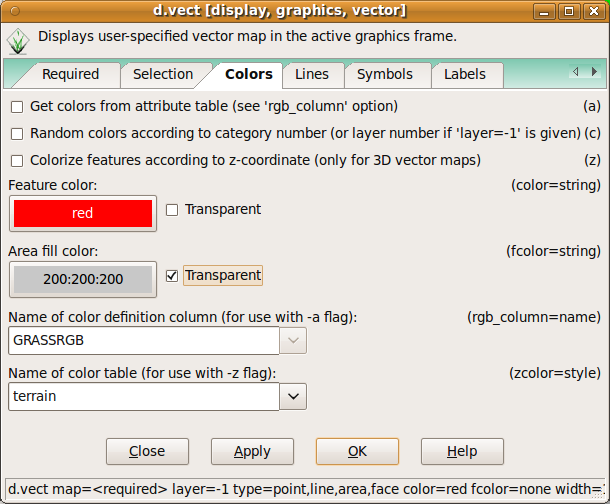
\includegraphics[width=0.5\textwidth]{./images/wxGUI_2.png}
    \caption{Module dialog generated for \module{d.vect}}
    \label{fig:wxGUI2}
    \end{subfigure}
\caption{Core wxGUI components}
\label{fig:wxGUI}
\end{figure}

Apart from the core components, there are additional tools available.
These are either integrated into Layer Manager or Map Display
(e.g.\ Vector Digitizer, 2.5D/3D visualization tool wxNviz) or they are in separate windows
(e.g.\ Cartographic Composer, Supervised Classification Tool, Profile Analysis Tool).

\section{Temporal data support and visualization}
The support of the temporal component of spatio-temporal data in GRASS is limited
(considering the situation before the integration of the Temporal Framework).
It is possible to assign a time stamp to a raster, vector or 3D-raster map using module
\module{r.timestamp}, \module{v.timestamp} and \module{r3.timestamp}, respectively.
These modules internally use \emph{GRASS Datetime Library} \cite{grassProgMan}.
However, time stamps serve only for information as a part of metadata.

Another module which can be used to process spatio-temporal data is \module{r.series}
which computes aggregate values from a series of raster maps. This is useful for example
for creating monthly average temperature maps from daily average temperature maps.

\subsubsection{Visualization}
\label{sec:grassVisualization}
Considering the visualization of spatio-temporal data, GRASS GIS offers
several possibilities.

\paragraph{Animation: xganim module} Module \module{xganim} is a tool for animating a series of raster maps.
This tool suffers from many problems which led to the development
of a better tool (described in section \ref{sec:animationTool}).

Module \module{xganim} in GRASS 7 is written in C++ using wxWidgets graphical toolkit.
This is inconsistent with the rest of wxGUI which is written in wxPython.
Originally, it was a X/Motif application, however in GRASS 7 it was necessary
to rewrite it because it was decided to leave the old display architecture.
It is apparent from the figure \ref{fig:xganim} that the GUI lags behind modern GUI design,
however, there are more serious problems.

\begin{figure}[ht!]
\centering
    \begin{subfigure}[ht]{0.49\textwidth}
    \centering
        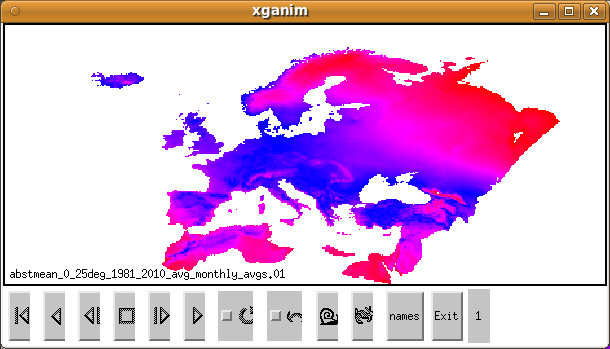
\includegraphics[width=\textwidth]{./images/xganim64.png}
    \caption{\module{xganim} in GRASS 6}
    \label{fig:xganim6}
    \end{subfigure}
    \begin{subfigure}[ht]{0.49\textwidth}
    \centering
        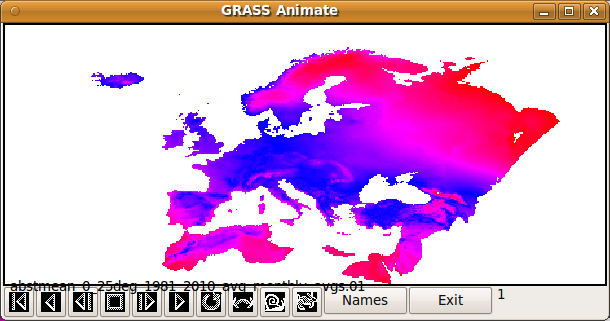
\includegraphics[width=\textwidth]{./images/xganim7.png}
    \caption{\module{xganim} in GRASS 7}
    \label{fig:xganim7}
    \end{subfigure}
\caption{Screenshot of \module{xganim} tool in different versions of GRASS}
\label{fig:xganim}
\end{figure}

One of the problems is that the speed of the animation is very difficult to control.
This is the result of the rather primitive implementation of the part
responsible for changing frames at the right time.
Frames are changed in response to emitted events.
These events are emitted when system becomes idle which the programmer is not able to affect.
Moreover, the delay between two successive frames is implemented as a for loop
and to change the speed of the animation the number of loops is increased or decreased.
Therefore the default speed of the animation on the current computers
is much faster than it used to be ten years ago.

Also, such tool should offer a way to explore raster series more interactively.
For example, it lack a slider control (or any other similar widget)
which enables to browse the raster maps easily and in an intuitive way.


\paragraph{Animation: m.nviz.image}
Module \module{m.nviz.image} is not really an animation tool as \module{xganim} module described above,
however it can be used to create an animation.
The purpose of this module is to render 3D view of raster, vector or 3D raster date to an image.
The underlying library, \emph{OGSF}, is used by both \module{m.nviz.image}
and the interactive 3D view tool\,---\,wxNviz (mentioned below).
Module \module{m.nviz.image} as a command line tool is ideal for scripting.
Typically, \module{m.nviz.image} is run in a loop while one or more parameters change.
The resulting sequence of images can be converted to an animation by an external program,
e.g.\ \emph{ImageMagick}\footnote{\url{http://www.imagemagick.org/}} or
\emph{FFmpeg}\footnote{\url{http://ffmpeg.org/}}.

Because it is not easy to specify the optimal parameter values
(especially view parameters) it is recommended to first find best view using interactive
wxNviz and then use its ability to generate the command for \module{m.nviz.image} for the current state.
This command can be than edited and used in a script.
Follows an example of a simple Bash script which creates a video from raster series (mapset NagsHead\_series).


\begin{small}
\begin{lstlisting}[style=mybash]
IMG=img
let NUM=0
for map in `g.mlist type=rast pattern=NH_* sep=" " --q`
do
    let NUM++
    m.nviz.image elevation_map=$map format=tif \
    output=${IMG}_$NUM zexag=4 persp=12 height=300
done
ffmpeg -sameq -r 5  -i ${IMG}_%d.tif output.avi
\end{lstlisting}
\end{small}



\paragraph{Space-Time Cube: wxNviz}
WxNviz, originally Nviz, is 2.5D/3D visualization tool which is able to render
multiple surfaces (rasters) in 3D, display 3D vector data and voxel data (3D raster).
There is no direct support for temporal data yet, however it can be 
used for the visualization of space-time cube.

The approach described in \ref{voxelHelena} requires to create voxel data
where the $z$ coordinate represents time.
This can be achieved by using \module{r.to.rast3} \cite{grassUserMan}
which converts series of 2D raster maps to one 3D raster map as illustrated in figure \ref{fig:rtorast3}.

\begin{figure}[h!]
  \centering
  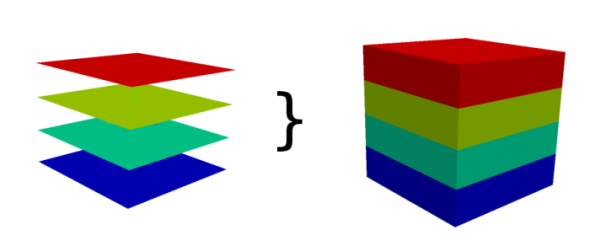
\includegraphics[width=0.7\textwidth]{./images/rtorast3.png}
  \caption[Functionality of module \module{r.to.rast3}]
  {Functionality of module \module{r.to.rast3}. Source: GRASS GIS 7.0 Reference Manual \cite{grassUserMan}.}
  \label{fig:rtorast3}
\end{figure}

In case we have vector points data (e.g.\ LiDAR data), module \module{v.vol.rst} interpolates these points into a 3D raster
map using regularized spline tension algorithm (RST) \cite{mitasova1993interpolation,mitasova1993interpolation2}.

Having the voxel data, we can visualize them in 3D view as isosurfaces
or cross-sections. An isosurface is an analogue of an isoline in 3D.
In the figure \ref{fig:nviz_isosurface} displaying elevation voxel data%
\footnote{available from \url{http://courses.ncsu.edu/mea582/common/media/01/NagsHead_series.zip}},
isosurface represents the change of a particular contour line in time.
The movement of the contour is apparent from the changing shape of the isosurface.
Also, time component can be emphasized by a color scheme which can better identify the time when changes occur.
The same changes in elevation can be inferred from the cross-sections visualization (figure \ref{fig:nviz_slices})
where the cross-section is an intersection of a plane with the voxel cube.
These techniques are used by Mitasova TODO ref Visualizations of Coastal Elevation Time-series




\begin{figure}[ht!]
\centering
    \begin{subfigure}[ht]{0.49\textwidth}
    \centering
        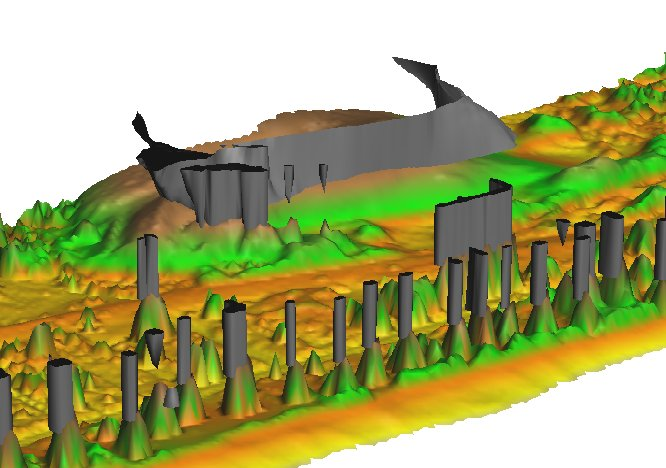
\includegraphics[width=\textwidth]{./images/nviz_isosurface.jpg}
    \caption{isosurface}
    \label{fig:nviz_isosurface}
    \end{subfigure}
    \begin{subfigure}[ht]{0.49\textwidth}
    \centering
        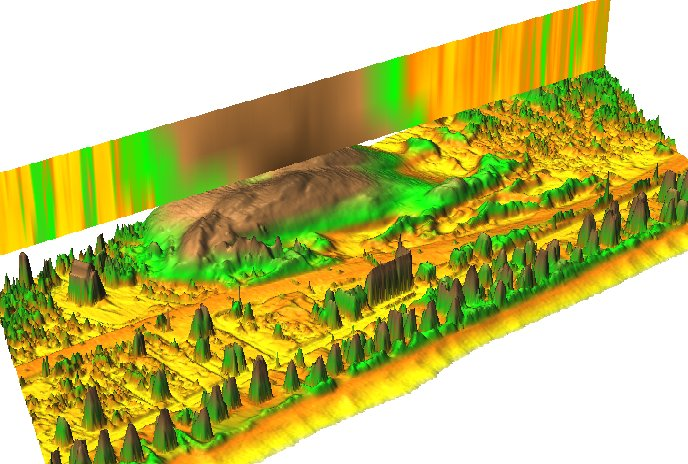
\includegraphics[width=\textwidth]{./images/nviz_slices.jpg}
    \caption{cross-section}
    \label{fig:nviz_slices}
    \end{subfigure}
\caption[Visualization of 3D raster (voxel) data of elevation with $z$ coordinate as time in GRASS GIS]
{Visualization of 3D raster (voxel) data of elevation with $z$ coordinate as time in GRASS GIS.
Figure \subref{fig:nviz_isosurface} shows an evolution of a contour line ($z=10\ m$).
A cross-section on figure \subref{fig:nviz_slices} also illustrates that the height of the middle
part changed with time.
Data source: mapset NagsHead\_series}

\label{fig:nviz_voxel}
\end{figure}



% http://courses.ncsu.edu/mea582/common/media/01/NagsHead_series.zip

\section{Temporal GRASS GIS framework}
\label{sec:GRASSTF}
Temporal GRASS GIS Framework is a new extension available in GRASS 7
for manipulating spatio-temporal data \cite{soerenTGRASS}.
It enables to manage, analyze and process large amount of spatio-temporal data.
Following the GRASS GIS modular design, the framework introduces over 30 new modules.
Temporal modules' names starting with t./t.rast/t.vect/t.rast3d names
comply with the GRASS modules' naming conventions.

\subsection{Implementation}
\tf uses a snapshot approach (described above).
This approach can be easily understood and is simple enough to be integrated into the layer-based GIS.
The integration consists of two levels.
In the first level, timestamps are assigned to the existing spatial data types -- raster, vector, 3D raster maps.
The second level introduces new datatypes -- space time raster,
vector and 3D raster datasets (referred as stdrs, stvds and str3ds).

The implementation of the \tf is based on a temporal library and a SQL database scheme.
The library is written in Python programming language and provides an application programming interface (API) which is used by the temporal modules,
however the library is meant to be used not only by other modules but also within user scripts or the GRASS GUI if needed.
Beside valid time the temporal database stores also transaction time%
\footnote{Valid time is the time period during which a database fact is valid in the modeled reality,
transaction time  is the time period during which a database fact is stored in the database \cite{temporalGlossary}}
and other map and dataset metadata.
The \tf supports two different database back-ends -- SQLite%
\footnote{\url{http://www.sqlite.org/}} (more lightweight) and
PostgreSQL\footnote{\url{http://www.postgresql.org/}}.
However, GRASS GIS users usually do not have to come in contact with the underlying database backend
as the default SQLite driver is often what they need.

\subsection{Basic concepts}
The \tf follows the concept of linear and discrete time.
To understand the basic concept of the \tf it is necessary to explain several terms.
The terms are explained in the context of the \tf , more theoretical and accurate definitions can be found in \cite{temporalGlossary}.

\paragraph{Interval vs. point time}
\label{sec:intervalVsPoint}
One can decide which time model to use -- interval time or time instances (also called point time).
Point time is a single moment in the time dimension
while interval is a period of time consisting of two instances -- start time instance and end time instance.
The time interval contains the start time but not the end time:
$$[start, end)$$

Each type is suitable for different types of data.
Consider temperature and precipitation measuring.
While temperature is measured in a given time instance and the measured value describes the state,
precipitation is measured over a given time period. The decision which model to choose is not always
straightforward, however it appears that for many applications,
interval time is a better choice \cite{pointVsInterval}.

\paragraph{Absolute vs. relative time}
\label{sec:absoluteVsRelative}
Absolute time stamp is related to a fact and it does not depend on any other facts.
On the contrary, relative time is related to another time and
it can be represented even by a negative number which stands for ``before".
The \tf recognizes several date time formats for absolute time -- TODO.
Relative time format consists of a number and time unit, which can be one the following: \emph{years},
\emph{months}, \emph{days}, \emph{hours}, \emph{minutes} and \emph{seconds} (see table \ref{tab:timeFormat}).

\begin{table}[ht!]
  \centering
\caption{Examples of valid time formats}
\label{tab:timeFormat}
\setlength{\extrarowheight}{3pt}
\begin{tabular}{|l|l|}
\hline
\multirow{3}{*}{Absolute time}
 & 2001-01-05  \\ \cline{2-2}
 & 1996-07-06 23:01:59  \\\cline{2-2}
 & TODO  \\
 \hline
\multirow{2}{*}{Relative time}
 & 1 months  \\\cline{2-2}
 & -5 years  \\
 \hline
\end{tabular}
\end{table}

\paragraph{Temporal granularity}
\label{sec:temporalGranularity}
Temporal granularity is an important characteristics of every temporal dataset.
In the context of the \tf , it represents the greatest common divisor
of the temporal extents (and possible gaps) of all maps of the dataset.
The temporal granularity can change every time there is a change in dataset maps
(added, removed or changed time stamp).
To understand better, see table \ref{tab:granularity} content of which is based on the output
of one of the temporal modules (namely \module{t.rast.list}).

Example interval time dataset consists of 6 maps and
there are also two gaps which means that at this time period no data are available.
The column \emph{Duration} contains the number of days for each period and it can be inferred
that the greatest common divisor is 2 months.
\begin{table}[ht!]
  \centering
  \caption{Example dataset}
  \label{tab:granularity}
\setlength{\extrarowheight}{3pt}
\begin{tabular}{cccr}
\toprule
 Map name & Start time & End time & Duration [days]\\\midrule
avg\_temp.01@timeseries &    2001-01-01 00:00:00  &   2001-03-01 00:00:00  &   59.0\\
avg\_temp.02@timeseries  &  2001-03-01 00:00:00  &   2001-05-01 00:00:00   &  61.0\\
no map (gap)    &  2001-05-01 00:00:00    & 2001-09-01 00:00:00   &  123.0\\
avg\_temp.03@timeseries     & 2001-09-01 00:00:00   &  2001-11-01 00:00:00  &   61.0\\
no map (gap) &   2001-11-01 00:00:00   &  2002-01-01 00:00:00  &   61.0 \\
avg\_temp.04@timeseries  &    2002-01-01 00:00:00   &  2002-05-01 00:00:00     & 120.0 \\
avg\_temp.05@timeseries  &      2002-05-01 00:00:00 &    2002-07-01 00:00:00 &    61.0 \\
avg\_temp.06@timeseries &     2002-07-01 00:00:00  &   2002-09-01 00:00:00   &  62.0\\
\bottomrule
\end{tabular}
\end{table}


\paragraph{Temporal topology}
\label{sec:temporalTopology}
Although topology is a term widely used in the area of mathematics studying properties of space,
this term can be used analogically for the time dimension.
Temporal topology analyzes temporal relations between time stamps (for both interval and point time).
There are 13 base relations between two intervals according to \cite{relationships}.
Table \ref{tab:relationships} shows these relations (without the inverse relations).


\begin{table}[ht]
\centering
\caption{Temporal relationships according to \cite{relationships}}
\label{tab:relationships}
\setlength{\extrarowheight}{10pt}

% \setlength{\unitlength}{5cm}
% \linethickness{5mm}
\begin{tabular}{|p{6.5cm}|l|}

\hline
\intervals{0cm}{2cm}{3cm}{2cm} \vspace{5pt} &  X before Y   \\\hline
\intervals{0cm}{2cm}{2cm}{2cm} \vspace{5pt} &  X meets Y \\\hline
\intervals{0cm}{3cm}{2cm}{3cm} \vspace{5pt} &  X overlaps with Y  \\\hline
\intervals{0cm}{3cm}{0cm}{5cm} \vspace{5pt} &  X starts Y  \\\hline
\intervals{1cm}{3cm}{0cm}{5cm} \vspace{5pt} &  X during Y  \\\hline
\intervals{2cm}{3cm}{0cm}{5cm} \vspace{5pt} &  X ends Y  \\\hline
\intervals{0cm}{5cm}{0cm}{5cm} \vspace{5pt} &  X equal Y   \\\hline

\end{tabular}
\end{table}

The topology of a temporal dataset can be valid or invalid which depends on the relationship between dataset maps.
If certain maps overlap or one is contained by the other then the dataset has invalid topology.
As a consequence, such dataset is not accepted by certain temporal modules.

\paragraph{Temporal sampling}
\label{sec:temporalSampling}
Temporal sampling is used to determine the state of one process during a second process.
The \tf enables to sample a dataset (can have both point and interval time) by another dataset having interval time.
There is an example of temporal sampling in figure \ref{fig:samplingExample}.
The figure indicates that for different sampling methods (temporal relationships)
which are provided by module \module{t.sample}, different results are expected.

In figure \ref{fig:samplingExampleReverse}, the input (sampled) dataset and the sample dataset are interchanged
to demonstrate the reciprocity of the temporal relations. For example, the table \ref{fig:samplingTable} shows that
there is a relation \emph{during} between intervals $Y_2$ and $X_2$, $X_3$.
When the same datasets are interchanged the relation must remain, however it is transformed into \emph{contain}.
The same applies for relations \emph{precede} and \emph{follow}.
Relation \emph{equal} does not have any opposite relation and \emph{overlap} involves both cases (\emph{overlap, overlapped}).
The opposite of the relation \emph{start} is \emph{end} which is not included in \module{t.sample} options.



\begin{figure}[ht]
\centering
    \begin{subfigure}[ht]{\textwidth}
    \centering
    \setlength{\unitlength}{1cm}
        \begin{tabular}{ll}
            Sampled dataset & \framebox[3cm][c]{$X_1$}\framebox[1cm][c]{$X_2$}\framebox[2cm][c]{$X_3$}\framebox[3cm][c]{$X_4$} \\
            & \\
            Sample dataset & \rule{1cm}{0cm}\framebox[1cm][c]{$Y_1$}\framebox[4cm][c]{$Y_2$}\framebox[3cm][c]{$Y_3$} \\
            & \hspace{1cm}\raisebox{3pt}{\thicklines \vector(1, 0){5}} time \\

        \end{tabular}
    \label{fig:samplingDatasets}
    \caption{Space time datasets with interval time}
    \end{subfigure}
    
\vspace{0.5cm}
    \begin{subfigure}[ht]{\textwidth}
    \centering
    \setlength{\extrarowheight}{3pt}
        \begin{tabular}{c|c|c|c|c|c|c|c|}
              & start & during & contain & overlap & equal &follow &precede\\\hline
        $Y_1$ & --- & --- & $X_1$ & --- & ---&--- &---\\
        $Y_2$ & $X_2$, $X_3$ & $X_2$, $X_3$ & --- & $X_1$ & ---& $X_4$&--- \\
        $Y_3$ & $X_4$ &---  & --- & --- & $X_4$& ---&$X_3$
        \end{tabular}
    \caption{Sampling result for each temporal relationship}
    \label{fig:samplingTable}
    \end{subfigure}

\caption{Example of space time dataset sampling }
\label{fig:samplingExample}
\end{figure}


\begin{figure}[ht]
\centering
    \begin{subfigure}[h]{\textwidth}
        \centering
        \setlength{\unitlength}{1cm}

        \begin{tabular}{ll}
            Sampled dataset & \rule{1cm}{0cm}\framebox[1cm][c]{$Y_1$}\framebox[4cm][c]{$Y_2$}\framebox[3cm][c]{$Y_3$} \\
            & \\
            Sample dataset & \framebox[3cm][c]{$X_1$}\framebox[1cm][c]{$X_2$}\framebox[2cm][c]{$X_3$}\framebox[3cm][c]{$X_4$}\\
            & \hspace{1cm}\raisebox{3pt}{\thicklines \vector(1, 0){5}} time \\
        \end{tabular}
        \label{fig:samplingDatasetsReverse}
        \caption{Space time datasets with interval time (switched datasets from figure \ref{fig:samplingExample})}
    \end{subfigure}

\vspace{0.5cm}
    \begin{subfigure}[h]{\textwidth}
    \centering
    \setlength{\extrarowheight}{3pt}
        \begin{tabular}{c|c|c|c|c|c|c|c|}
            & start        & during & contain & overlap & equal &follow &precede\\\hline
        $X_1$ & $Y_1$, $Y_2$ & $Y_1$  & ---     & $Y_2$   & ---   &---    &---\\
        $X_2$ & ---          & ---    & $Y_2$   & ---     & ---   & ---   &--- \\
        $X_3$ & ---          & ---    & $Y_2$   & ---     & ---   & $Y_3$ &--- \\
        $X_4$ & $Y_3$        &---     & ---     & ---     & $Y_3$ & ---   &$Y_2$
        \end{tabular}
    \label{fig:samplingTableReverse}
    \caption{Sampling result for each temporal relationship}
    \end{subfigure}
\caption{Example of space time dataset sampling (switched sampled and sample dataset)}
\label{fig:samplingExampleReverse}
\end{figure}



\subsection{Functionality}
The temporal library provides wide functionality which is accessible either via Python API or GRASS temporal modules.
The main capabilities of the library include:

\begin{itemize}
    \item Registration of raster, vector a 3D raster maps in datasets (called \emph{strds}, \emph{stvds}, \emph{str3ds}, respectively).
    \item Support of absolute and relative time (only maps of one type can be in one dataset).
    \item Support of interval and point time (can be used together in one dataset).
    \item Metadata (number of maps, spatial, temporal extent, creation time, \ldots) of a dataset
    are recomputed automatically after (un)registering of maps.
    \item Computation of time granularity.
    \item Computation of temporal topology and reporting its validity.
    \item Temporal sampling of one dataset by another dataset or by its time granularity.
\end{itemize}

Other functionality needed for handling spatio-temporal data is provided by temporal modules.
The integration of the framework into GRASS GIS enables the \tf to reuse existing
functionality to process spatial data.

Temporal modules share certain common options:
\begin{itemize}
  \item They allow to specify the temporal range of datasets so that only a part of a dataset can be processed.
  \item Several modules support two possibilities of specifying the input data\,---\,directly or by providing a file.
  \item When modules output a report or a table it is possible to change the format suitably.
\end{itemize}

The important ability of the \tf is the interoperability
with several powerful open-source applications for statistical computations and visualization.
Textual ouputs of many modules are suitable for statistical environment \emph{R}\footnote{\url{www.r-project.org/}}.
Module \module{r3.out.netcdf} exports 3D raster to NetCDF
format\footnote{\url{http://www.opengeospatial.org/standards/netcdf}}
which can be then processed e.g. in \emph{Climate Data Operator (CDO)}\footnote{\url{https://code.zmaw.de/projects/cdo}}.
The support of visualization software \emph{ParaView}\footnote{\url{http://www.paraview.org/}} is available
through VTK format which can be exported by temporal module \module{t.rast.out.vtk}.




% TODO: space time voxel cubes



\chapter{Results}%Developed visualization tool
\label{chap:results}
The new \tf brings new possibilities to process spatio-temporal data,
however it is not focused on its visualization in GRASS GIS. To partially fill this `missing gap',
three new tools have been developed which either make use of the \tf
or help to explore spatio-temporal data generally.

These tools are:
\begin{description}
    \item[\at]for animation of raster map series or space time raster dataset, both in 2D and 2.5D.
    \item[Timeline Tool] as a support tool for visualization of dataset's topology and other metadata.
    \item[\ms]for a comparison of two raster maps of the same area from different time period.
\end{description}

\section{Animation tool}
\label{sec:animationTool}
As described in section \ref{sec:mapAnimation},
animation is a natural and easily understandable way to display spatio-temporal data.

Because the current animation module \module{xganim} was very limited
in several aspects (explained in section \ref{sec:grassVisualization}),
a new tool has been developed.
Screenshots of the \at can be found in appendix \ref{appdx:animation}.

\subsection{Features}
Beside the features of \module{xganim} module, \at provides new possibilities
to explore spatio-temporal data.

Basic features (also existing in \module{xganim} module):
\paragraph{More views}
\at can display up to 4 different synchronized animations at once.
Unlike the \module{xganim} module, it is possible to add or remove each of the views separately
without the need to restart it.
\paragraph{Change animation speed}
Unlike the \module{xganim} module where you can only
slow down or speed up the animation by an unspecified coefficient, \at allows to set
exact duration of the frame (in milliseconds).
\paragraph{Loops}
There are two methods of looping key frames.
The first type cycles through the key frames and when it reaches the last one it jumps back
to the first key frame and continues looping.
The second type of looping goes back through the key frames in reverse order.


New features:
\paragraph{Interactive change of the active frame}
In order to better control currently displayed frame a slider control is provided.
By dragging the slider's knob user can select a certain frame.
Also it enables to inspect in detail a part of an animation
by repeated dragging of the knob back and forth within a few frames.
      
\paragraph{Support of the \tf}
The most important attribute of the \at is the interoperability with the \tf
which involves several features described in section \ref{sec:wx.animation:support}.
      

\paragraph{3D view animation}
A nice feature is the ability to animate raster maps in 3D view.
As illustrated in figure \ref{fig:color_elevation_map},
raster maps can either represent a changing color of a static surface (\subref{fig:color_map}) or
a changing surface (\subref{fig:elevation_map}).
Apart from raster maps, also vector point and line data can be animated, too.
Implementation details can be found in section \ref{sec:3dViewAnimation}.

\begin{figure}[ht]
\centering
    \begin{subfigure}[h]{\textwidth}
    \centering
    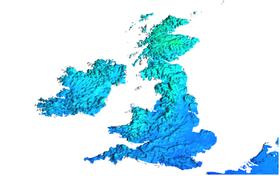
\includegraphics[width=0.3\textwidth]{./images/color_map1.png}
    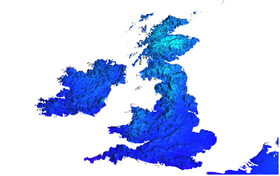
\includegraphics[width=0.3\textwidth]{./images/color_map2.png}
    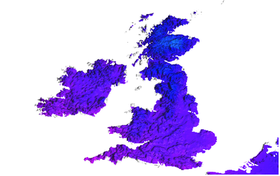
\includegraphics[width=0.3\textwidth]{./images/color_map3.png}
    \caption{Change of color map (temperature)}
    \label{fig:color_map}
    \end{subfigure}
    
    \begin{subfigure}[h]{\textwidth}
    \centering
    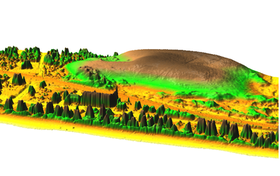
\includegraphics[width=0.3\textwidth]{./images/elevation_map1.png}
    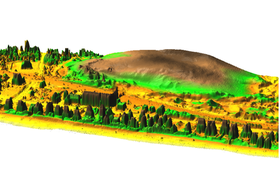
\includegraphics[width=0.3\textwidth]{./images/elevation_map2.png}
    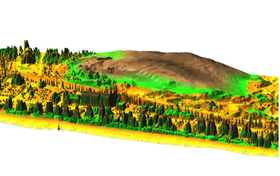
\includegraphics[width=0.3\textwidth]{./images/elevation_map3.png}
    \caption{Change of elevation map (Nags Head area)}
    \label{fig:elevation_map}
    \end{subfigure}
    \caption{Example}
    \label{fig:color_elevation_map}
\end{figure}

        
      
\paragraph{Export}
Animation can be exported either as a sequence of images or an animated gif.
%TODO: add example of ffmpeg command
Sequence of images can be converted to a video file in several ways.
One of the possibilities is to call ffmpeg\footnote{\url{http://ffmpeg.org/}} with the following parameters
      
\begin{footnotesize}
\begin{lstlisting}[style=mybash]
ffmpeg -r 10 -i input_%02d.png -sameq -vcodec mpeg4 output.avi
\end{lstlisting}
\end{footnotesize}
      where \emph{-r} stands for frame rate (frames per second),
      \emph{-i} for input files (requires sequential numbering of files) and
      \emph{vcodec} determines the video encoding.
      The export dialog provides the user with the frame rate, so that he can then create
      a video with the same frame rate%
      \footnote{However, not all video codecs and containers support an arbitrary frame rate.} as in the \at.

      A usual requirement is include some additional text, logo or time stamp in the video.
      The \at supports all these options, moreover the number of these decorations is not limited.
      The placement is specified as the percentage of the image size from the top left corner.
      

\subsection{Support of the \tf}
\label{sec:wx.animation:support}
The \at supports the \tf in several ways. Certain features use the \tf in a more complex way than the others.

The \at accepts space time raster dataset as an input. By the means of the \tf, it determines the maps which are then loaded.
Apart from that, also multiple raster maps are accepted directly.

However, the main difference between displaying a set of maps and a space time dataset is
that the duration of each key frame is given by the given time stamp information.
This is useful when data are collected in irregular intervals.
Then, the key frames do not change e.g.\ every second but at a given moment the frame stays visible for a longer time.
To achieve similar behavior it is necessary to add the frame multiple times, see figure \ref{fig:temporalDifference}.
Concerning temporal data having interval time, there are cases when no data were collected or measured at all.
The \at recognizes such cases and displays a ``no data'' sign in order to make the user aware of the gap in data.

\begin{figure}[ht]
  \centering
\framedInterval{2.5cm}{$X_1$}{(2001, 2002]}%
\framedInterval{5cm}{$X_2$}{(2002, 2004]}%
\framedInterval{2.5cm}{$X_3$}{(2004, 2005]}%

\framedInterval{2.5cm}{$X_1$}{}%
\framedInterval{2.5cm}{$X_2$}{}%
\framedInterval{2.5cm}{$X_2$}{}%
\framedInterval{2.5cm}{$X_3$}{}%

\caption{Difference in animations of temporal data and non-temporal data collected at irregular intervals}
\label{fig:temporalDifference}

\end{figure}

In case of loading more space time datasets the \tf enables to synchronize the animations
even if the temporal datasets are spaced unequally.
Figure \ref{fig:synchronizedAnim}) presents an example of such datasets and the related table
shows the frames displayed at selected time instances.
The concept of temporal granularity and temporal sampling is used to achieve this described behavior.


\begin{figure}[ht]
\centering
\begin{minipage}{10cm}
\framedInterval{75pt}{$X_1$}{}%
\framedInterval{25pt}{$X_2$}{}%
\framedInterval{50pt}{$X_3$}{}%
\framedInterval{100pt}{$X_4$}{}%

\framedInterval{25pt}{$Y_1$}{}%
\framedInterval{100pt}{$Y_2$}{}%
\framedInterval{25pt}{$Y_3$}{}%
\framedInterval{50pt}{$Y_4$}{}%

\vspace{10pt}

\hspace{-3pt}$\uparrow$\hspace{45pt}$\uparrow$\hspace{45pt}$\uparrow$\hspace{93pt}$\uparrow$

\hspace{-3pt}$t_1$\hspace{45pt}$t_2$\hspace{40pt}$t_3$\hspace{90pt}$t_4$
\end{minipage}

\bigskip

\begin{tabular}{lcc}
\toprule
Time & Animation X & Animation Y \\ \midrule
$t_1$ & $X_1$& $Y_1$\\
$t_2$ & $X_1$& $Y_2$\\
$t_3$ & $X_3$& $Y_2$\\
$t_4$ & $X_4$& ---\\\bottomrule
\end{tabular}

\caption{Synchronized animations of space time datasets $X$ and $Y$}
\label{fig:synchronizedAnim}
\end{figure}

Datasets with interval and point time have to be distinguished.
Displaying interval data means to display each map (frame) for the time interval given by its start and end time.
However, point data have no end time. Therefore a different logic must be used to determine when each map should be displayed.
The \at treats point data as interval data where the end time of one map is the start time of the following map.

The time stamp information extracted from the dataset is presented to the user.
The format is given by the \emph{GRASS Datetime Library}. % which url too put here?
The support of other date time formats is planned.


\subsection{Usage}
There are two ways to launch the \at.
First option is to launch it from Layer Manager menu.
If there are any raster maps selected in the Layer Manager, the \at will load these maps automatically.
This simplifies the workflow of analyzing data as it is not necessary to specify maps several times.

Another option, which might appear more natural to many GRASS users,
is to launch the \at as a module from command line. By typing:

\begin{small}
\begin{lstlisting}[style=mybash]
> g.gui.animation
\end{lstlisting}
\end{small}

the \at is launched with no data loaded and the user is supposed to specify maps via the GUI.
Additionally, input data can be specified directly in the command line.
As of any other GRASS module, the parameters of \module{g.gui.animation} command can be retrieved by typing:

\begin{small}
\begin{lstlisting}[style=mybash]
> g.gui.animation --help

Description:
 Tool for animating a series of GRASS raster maps
 or a space time raster dataset

Usage:
 g.gui.animation [rast=name[,name,...]] [strds=name] [--verbose]
   [--quiet]

Flags:
 --v   Verbose module output
 --q   Quiet module output

Parameters:
   rast   Raster maps to animate
  strds   Space time raster dataset to animate
\end{lstlisting}
\end{small}

The command line interface does not allow the access to complete functionality of the \at.
The reason is that providing all functionality through command line parameters
would result in too complicated parameters.
Moreover, this simple interface should be sufficient for most cases.


\subsection{Implementation}
While \module{xganim} module was written in wxWidgets using C++ programming language (in GRASS 7),
the \at is written completely in wxPython using Python so that it can be better integrated into the GRASS wxGUI.
It uses \emph{GRASS Python Scripting Library} and \emph{GRASS Python Temporal Library} \cite{grassProgMan},
which is the integral part of the \tf. In the following paragraphs, some of the implementation issues are described.

\subsubsection{Loading data}
It is important to be aware of the fact that animation can consist of hundreds of maps.
Unfortunately, the mechanism of loading raster data in \module{xganim} could not be simply
rewritten into Python because of performance issues.
Therefore it was necessary to choose a different implementation.

If we try to use the \module{xganim} implementation, we encounter two main problems.
First, when loading data, the \emph{GRASS Raster Library} functions \cite{grassProgMan} are called.
In Python we could use ctypes to interface these methods,
however these methods can call exit function which causes a sudden end of the program.
This behavior is sufficient for a module but it is not suitable for a long running GUI application.
Secondly, the image representing the raster map is created by setting the color of each pixel sequentially.
For this kind of operation, Python is too slow comparing to C or C++.
This problem can be alleviated by using NumPy\footnote{\url{http://numpy.scipy.org/}},
however that makes the code less readable.

One possible solution is to use the current system used by wxGUI
where the raster maps are rendered into temporary files by module \module{d.rast}.
However, this method is quite slow mainly because it is necessary to write data to disk and read them afterwards.
Therefore, this method was rejected for the time being.
There have been efforts to improve the rendering implementation%
\footnote{see related ticket \url{http://trac.osgeo.org/grass/ticket/1719}}
and once it is implemented it will not be a problem to change it also in the \at.

Eventually, the raster rendering is done by \module{r.out.ppm}.
It can send image data to standard output and
thanks to the simplicity of the PPM format (Portable Pixmap Format%
\footnote{\url{http://netpbm.sourceforge.net/doc/ppm.html}}),
the data are directly (without saving to file) converted into the image displayed in the \at.
The advantage of this solution is that the demanding computation is done inside the module, thus in C.
Moreover, if the module fails for any reason, the application is able to handle such situation and continue.
Still, the achieved performance is worse comparing to \module{xganim}.
This is probably caused by the fact that each call of the module requires not negligible amount of time.
Table \ref{tab:comparisonTime} shows a performance comparison of the described methods.
The time measurement was done on one computer and each number is a sample mean computed from 5 measurements.
To make the measurement more objective, the \module{xganim} source code was slightly
changed by avoiding reporting messages which would slow the loading down.
The absolute numbers are not as important, however when we compare one with another,
we can see that the difference between the new implementation and the original one is not so significant.
Additionally, there is one important aspect which effects the loading duration
significantly for all implementations\,---\,the size of the map.
If we double the size of the image, we can expect the duration to increase four times.

\begin{table}[h]
  \caption{Time needed for loading a space time raster dataset containing 224 maps (800~$\times$~347~pixels)}
  \label{tab:comparisonTime}
  \centering
    \begin{tabular}{lrr}
    \toprule
    original xganim & 46 s & 100 \%\\
    calling \module{r.out.ppm} & 51 s & 111 \%\\
    \module{d.rast} rendering to file (wxGUI) & 67 s & 146\%\\
    \bottomrule

    \end{tabular}
\end{table}




\begin{comment}
244 maps
r.out.ppm
51.177767992
51.0374698639
51.213670969
51.17771101
51.2618360519
========
51.174

66.5165150166
65.1940889359
65.5398728848
72.5624401569
65.7088599205
=====
67.104

46.050000
46.260000
46.260000
46.060000
46.110000
========
46.148
\end{comment}

The images are stored internally as \verb|wx.Bitmap| \cite{wxPythonDoc} objects.
The number of bitmaps is not limited programmatically,
however in reality it is limited by the the size of the bitmaps and available RAM.
This is not an issue for usual animations today.

\subsubsection{Window resizing}
Every application has to react on the change of its frame size.
Unlike \module{xganim}, the \at is able to resize the displayed images to fit the new frame size.
However, the images are only rescaled, so it produces less quality images.
On the other hand, the rescaled images are sufficient and the advantage is that
the data do not have to be reloaded every time the user resizes the window.
In the application status bar a warning appears to make the user aware of the fact
that the displayed data should be reloaded.

\subsubsection{Specifying the displayed extent}
The displayed extent of the maps is determined by the computational region%
\footnote{This region defines the geographic area (and resolution) in which all raster analyses are done.}.
To change the displayed region, it is necessary to run module \module{g.region} and then reload data.
At this stage, any interactive zooming would be problematic.
The best option would be to reuse the wxGUI rendering system including zooming in order to avoid code duplication.
Unfortunately, reloading all maps in this way would be more time-consuming.
When the wxGUI rendering system becomes faster
it will hopefully be  possible to reuse this system completely.


\subsubsection{Temporal sampling}
Displaying animation of datasets with unequally spaced intervals or instances is not a simple task.
The \tf which supports the concept of temporal granularity and temporal sampling makes this task feasible.

There are a few computations needed to display the right maps at the right moments.
These steps are the same no matter if there are one or more space time datasets.
The first step is to get the time granularity.
The second step is the sampling of each dataset by the granularity using temporal relation \emph{start}.
This way we get all needed information about the time intervals (or instances) and the names of the maps.
The \at then puts all of this information together.

Table \ref{tab:exampleOfSamplingImpl} shows the result of temporal sampling of two sample space time datasets.
As we can see, the temporal granularity of the dataset $X$ (1 month) differs from the granularity of dataset $Y$ (2 months).
The common granularity (1 month) is in this case easy to compute.
This granularity is then used to sample both datasets (table \ref{tab:exampleOfSamplingImpl-2}).


\begin{table}
 \centering
\caption{Example of two space time datasets $X$ and $Y$ and the their sampling by temporal granularity 1 month.}
\label{tab:exampleOfSamplingImpl}
\begin{subtable}{0.4\textwidth}
    \centering
    \caption{List of maps and valid time intervals}
    \begin{tabular}{lll}
    \toprule
    $X$ & start time & end time \\
    \midrule
    $X_1$ & 2001-02-01 & 2001-03-01\\
    $X_2$ & 2001-03-01 & 2001-06-01\\
    $X_3$ & 2001-07-01 & 2001-10-01\\
    $X_4$ & 2001-10-01 & 2001-12-01\\
    \bottomrule
    \end{tabular}

    \vspace{20pt}
    \begin{tabular}{lll}
    \toprule
    $Y$ & start time & end time \\
    \midrule
    $Y_1$ & 2001-01-01 & 2001-03-01\\
    $Y_2$ & 2001-05-01 & 2001-07-01\\
    $Y_3$ & 2001-07-01 & 2001-09-01\\
    \bottomrule
    \end{tabular}
\end{subtable}
\quad
\begin{subtable}{0.4\textwidth}
\centering
\caption{Result of temporal sampling with granularity 1 month}
\label{tab:exampleOfSamplingImpl-2}
\begin{tabular}{llll}
\toprule
 $X$ & $Y$ & start time & end time \\\midrule
--- & $Y_1$ & 2001-01-01 & 2001-02-01\\
$X_1$& $Y_2$ & 2001-02-01 & 2001-03-01\\
$X_2$& --- & 2001-03-01 & 2001-04-01\\
$X_2$& --- & 2001-04-01 & 2001-05-01\\
$X_2$& $Y_2$ & 2001-05-01 & 2001-06-01\\
--- & $Y_2$ & 2001-06-01 & 2001-07-01\\
$X_3$& $Y_3$ & 2001-07-01 & 2001-08-01\\
$X_3$ &$Y_3$ & 2001-08-01 & 2001-09-01\\
$X_3$ & --- & 2001-09-01 & 2001-10-01\\
$X_4$& --- & 2001-10-01 & 2001-11-01\\
$X_4$ & --- & 2001-11-01 & 2001-12-01\\
\bottomrule
\end{tabular}
\end{subtable}

\end{table}

\subsubsection{Animation}
Animation basically means to display a sequence of images in the given time instances.
Crucial is to determine \emph{which} frame (map) and \emph{when} to display.
We first discuss the \emph{when}  and then the \emph{which} question.


The original \module{xganim} implementation of the animation is rather primitive
as explained in \ref{sec:grassVisualization}.
The \at implementation uses timer events (class wx.Timer provided by wxPython) to achieve regular time intervals between two frames.
The interval between two successive events is specified by the programmer according to what the user requires.
In case of space time datasets animation, the user specifies how long
should a chosen time unit\footnote{units of time supported by the \tf, section \ref{sec:absoluteVsRelative}}
last (in milliseconds).

For each dataset, there is a separate object which controls the animation.
These animation objects receive the timer events and determine
which frame to display according to the result of the temporal sampling explained above.
The timer interval represents the temporal granularity of the datasets.
Therefore, each map is displayed exactly at the right moment.

When the interval of a map takes more than one temporal granularity, internally, there is no redraw.



\subsubsection{Checking compatibility of data}
During the development it was necessary to decide which data are compatible and can be animated together.
Several combinations are possible.
\begin{description}
  \item[Space time dataset $\times$ multiple maps]
  This combination is allowed granted that the number of maps matches the number of maps in the dataset.
  Then, the animation behaves as if there was no temporal information.

  \item[Space time datasets with absolute $\times$ relative time]
  This case is not allowed because there is no obvious way to convert one type to another.

  \item[Space time datasets with interval $\times$ point time]
  This combination is allowed, however it might not behave as user expects.
  Therefore, there is a warning to make the user aware of this fact.
 \end{description}
 
In general, it is better to use data which are fully compatible to avoid confusion.
The \at always checks the user input and in the case it recognizes an incompatibility, it reports it to the user.


\subsubsection{3D view animation}
\label{sec:3dViewAnimation}
Images for 3D view animation must be first rendered by module \module{r.nviz.image} \cite{grassUserMan}.
The rendering is more time-consuming than loading raster maps for the 2D view,
however this does not affect the speed of the animation itself.

3D view animation requires to specify additional input data.
Beside the maps (either multiple maps or space time dataset), the user is asked for a \emph{workspace file}%
\footnote{Workspace file is XML file storing the state of the wxGUI application (e.g.\ loaded layers, displayed extent).}.
The workspace file has to be created during a GRASS wxGUI session with active 3D view,
so that it can provide information about the 3D view state. After parsing this file, a command for \module{m.nviz.image}
is created.
Additionally, the user chooses which parameter to animate.
Typically, it is either \emph{elevation\_map} or \emph{color\_map}
(see the difference between figures \ref{fig:color_map} and \ref{fig:elevation_map}),
although we can animate points or lines, too.

\subsection{Future development}
\begin{itemize}
  \item loading more layers
  \item add where to determine time interval
  \item add legend
  \item better support of formats
  \item 
\end{itemize}



\section{Timeline tool}
Timeline Tool is an interactive application based on wxPython and Python plotting library matplotlib \cite{matplotlib} which allows
the user of the \tf to visualize space time datasets' metadata, especially temporal and spatial extents.

\subsection{Features}
The main purpose of this tool is illustrated by the figure \ref{fig:timeline1}
which is the output plot generated by the tool.

The x-axis represents time and the space time datasets are located on y-axis.
This simple plot gives an immediate overview of the datasets' temporal extent.

Furthermore, it shows also other characteristics of the datasets.
Interval and point datasets are distinguished by different symbols (points and bars)
which is easily and intuitively understandable.
Datasets with relative and absolute time can be recognized by different x-axis tick labels (date/time format vs. integer).

Also, invalid topology of a dataset is visualized.
Invalid topology basically means overlaying intervals or points
which can be easily represented by using semi-transparency to draw plot.
As a result, overlaying intervals are darker
which allows to recognize them (see figure \ref{fig:timeline1}, red dataset topol\_abs8).

\begin{figure}[ht!]
  \centering
  \begin{subfigure}[ht]{\textwidth}
  \centering
  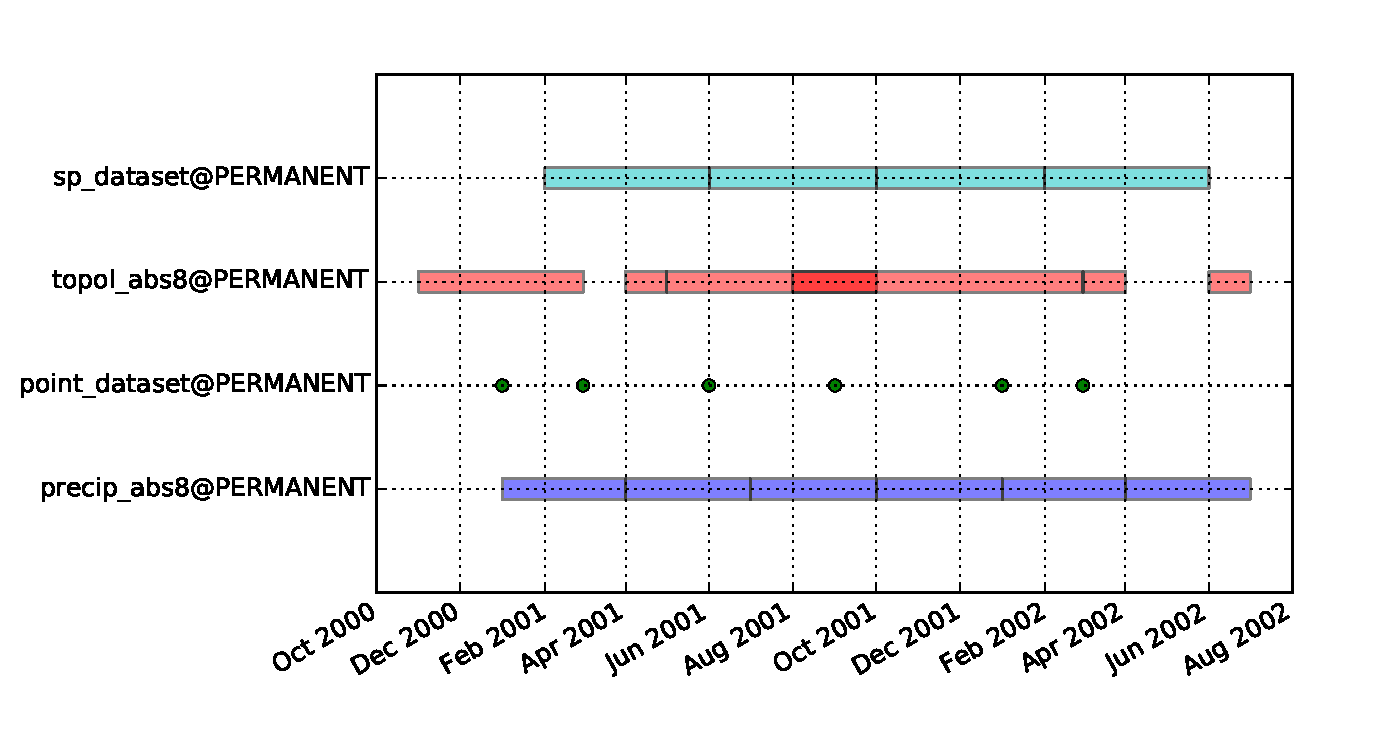
\includegraphics[width=0.8\textwidth]{./images/timeline1.pdf}
  \caption{temporal extents}
  \label{fig:timeline1}
  \end{subfigure}

  \begin{subfigure}[ht]{\textwidth}
  \centering
  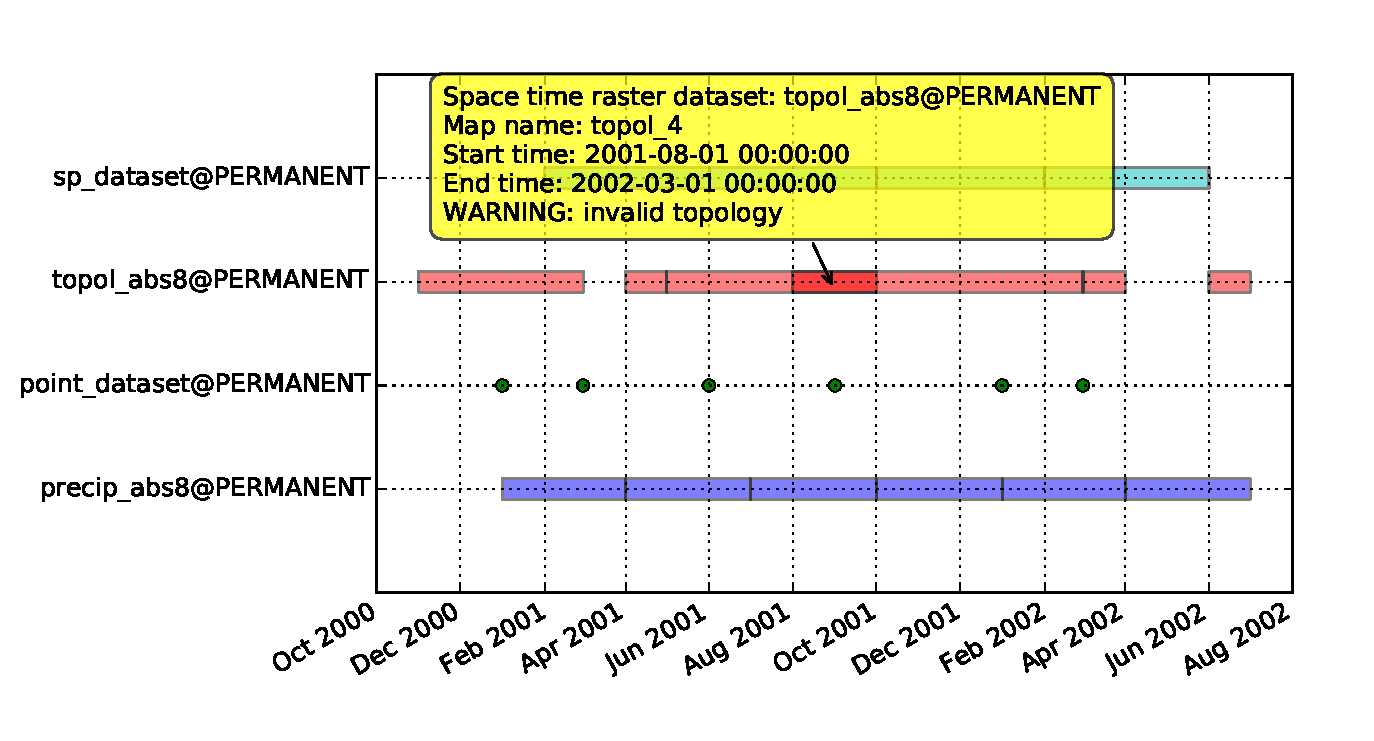
\includegraphics[width=0.8\textwidth]{./images/timeline3.pdf}
  \caption{annotation}
  \label{fig:timeline3}
  \end{subfigure}
%   
\caption{Timeline Tool: 2D plot of datasets' extents}
\label{fig:timeline}
\end{figure}

Other metadata can be displayed by clicking on the plotted dataset.
An annotation bubble appears showing basic information about the dataset and the selected map (figure \ref{fig:timeline3}).
It also warns about invalid topology of the dataset.


Not only temporal extent but also spatial extent can be visualized by using matplolib extension mplot3d.
The 3D plot is a space time cube where x- and y-axis represent the spatial part and the z-axis represents time (figure \ref{fig:timeline2}).

\begin{figure}[ht!]
  \centering
  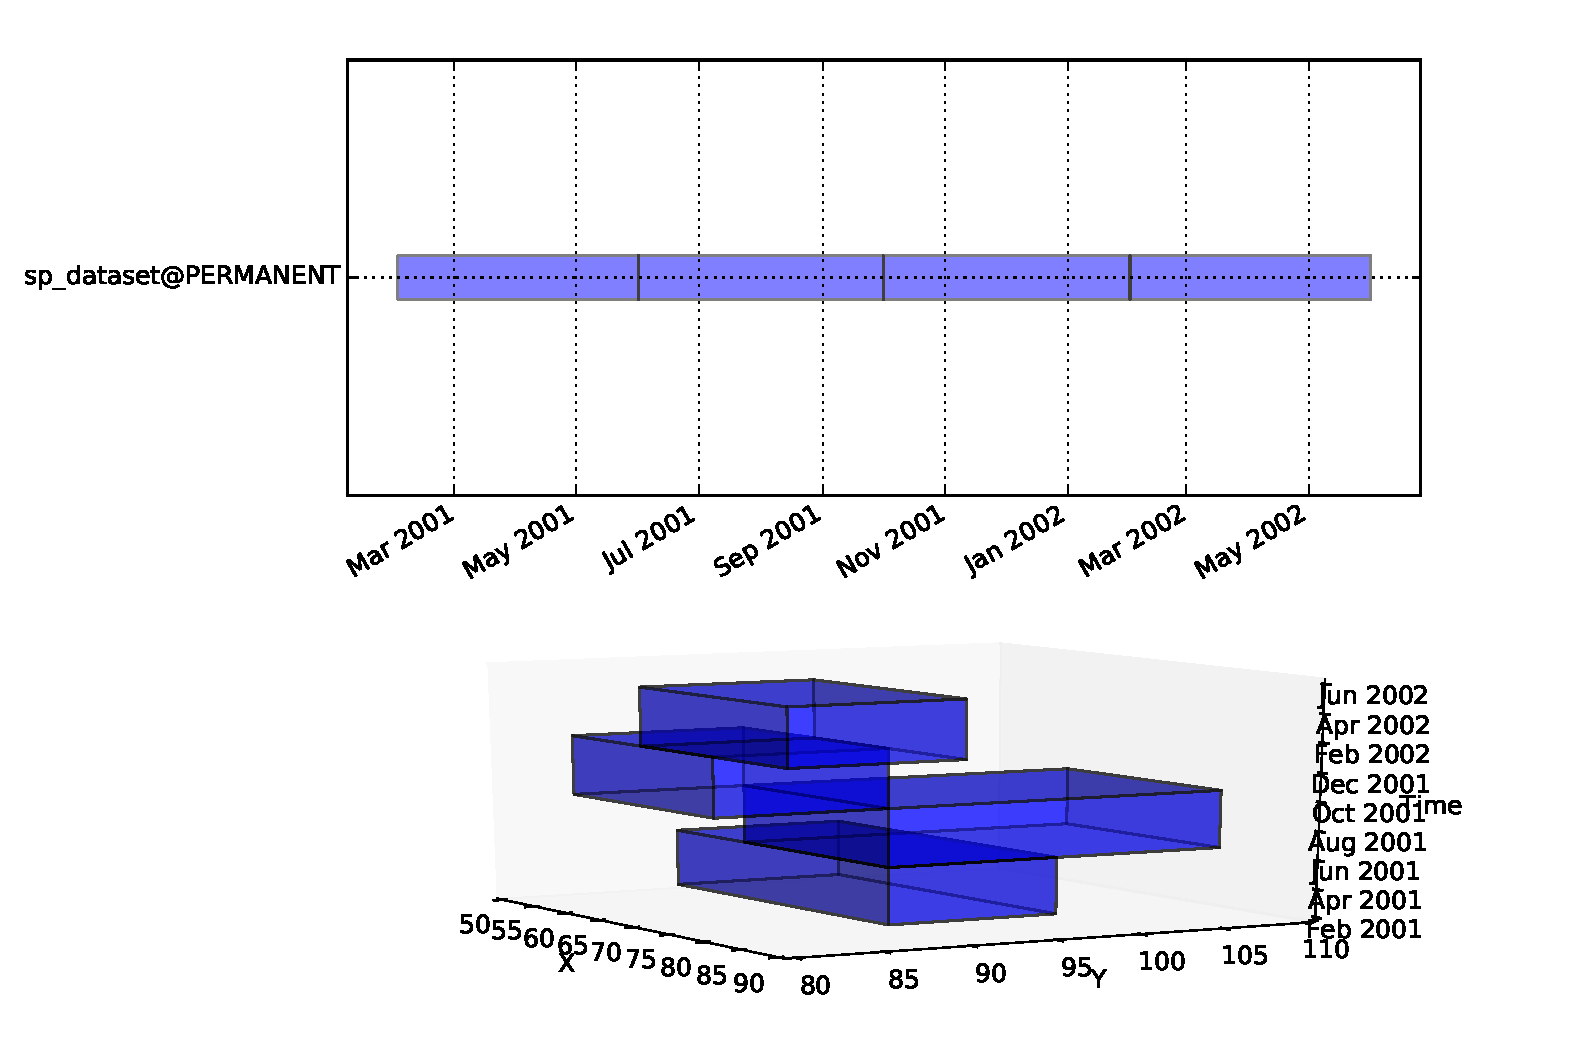
\includegraphics[width=0.8\textwidth]{./images/timeline2.pdf}
  \caption{Timeline Tool: spatial and temporal extents}
  \label{fig:timeline2}
\end{figure}

In order to better explore plotted data, the application allows to zoom,
pan (and in the case of the 3D plot also rotate) the plot.
This functionality is provided by matplotlib's navigation toolbar which is a great advantage both for programmers and users.
Moreover, this toolbar offers to export figure to various raster and vector formats.

\subsection{Implementation}
To achieve nice and interactive plots integrated into wxPython application, matplotlib was chosen as a best option.
Although matplotlib is not a required dependency for GRASS~7,
users often have this library already installed because of its usefulness and capabilities.
Another considered option was a wxPython module wx.lib.plot.
Despite the advantage that it is already a part of wxPython and thus, no other dependency would be required,
it lacks the ability to display time stamps as axis tick labels. This crucial functionality is available in matplotlib.

The Timeline Tool embeds matplotlib into wxPython program by using WXAgg backend.
This enables to integrate the figure canvas and the navigation toolbar
which provides zooming, panning and export functionality.
Beside this toolbar, the Timeline Tool has additional wxPython widgets to control user input.

Matplotlib is a Python library which is an active project and new versions are released approximately two times a year.
Unfortunately, this means that new versions can have different API and new functions unavailable in older versions.
This makes it hard or even impossible to provide the same functionality for all versions.
The Timeline Tool suffers from this problem, too.
The 3D functionality is not available for matplotlib versions older than 1.0.0 (January 2011)
because of slightly different API, the inability to easily combine 2D and 3D subplots in one figure
and the lack of support for alpha drawing.
The Timeline Tool was tested both with an older version 0.99.1 (available for Ubuntu 10.04) and the latest version 1.1.1.

The 3D functionality of matplotlib is still in development and there are many known problems%
\footnote{\url{http://matplotlib.org/mpl_toolkits/mplot3d/faq.html}}.
These issues will be hopefully fixed in future versions of matplotlib.
% Therefore, the Timeline Tool's 3D view is m


\subsection{Usage}
The Timeline Tool can be launched as any other GRASS module.
For displaying help, choose one of the following options:
\begin{small}
\begin{lstlisting}[style=mybash]
> g.manual entry=g.gui.timeline # opens manual page in a browser
\end{lstlisting}
\end{small}

\begin{small}
\begin{lstlisting}[style=mybash]
> g.gui.timeline --help

Description:
 Allows to compare temporal datasets
 by displaying their temporal extents in a plot.

Usage:
 g.gui.timeline [-3] [inputs=name[,name,...]] [--verbose] [--quiet]

Flags:
  -3   Show also 3D plot of spatio-temporal extents
 --v   Verbose module output
 --q   Quiet module output

Parameters:
  inputs   Name of the input space time datasets

\end{lstlisting}
\end{small}

The following example (from the test of \module{t.register} module)
can be run in the command line to test the Timeline Tool:
\begin{small}
\begin{lstlisting}[style=mybash]
# set and print the region first using r.mapcalc
g.region s=0 n=80 w=0 e=120 res=10 -p

# create e.g. 4 raster maps with random values
r.mapcalc --o expr="prec_1=rand(0,550)"
r.mapcalc --o expr="prec_2=rand(0,450)"
r.mapcalc --o expr="prec_3=rand(0,320)"
r.mapcalc --o expr="prec_4=rand(0,510)"
r.mapcalc --o expr="prec_5=rand(0,550)"
r.mapcalc --o expr="prec_6=rand(0,450)"
r.mapcalc --o expr="prec_7=rand(0,320)"
r.mapcalc --o expr="prec_8=rand(0,510)"

# create the space time raster dataset with absolute time
t.create --o type=strds temporaltype=absolute output=precip_abs1 \
title="A test" descr="A test"
t.create --o type=strds temporaltype=absolute output=precip_abs2 \
title="A test" descr="A test"

# register the raster maps in the first space time dataset
# with given start time and increment
t.register --o -i input=precip_abs1 \
maps=prec_1,prec_2,prec_3,prec_4 \
start="2001-01-01" increment="1 years, 10 days"

# register the raster maps in the second space time dataset
# with given start and end time
t.register --o -i input=precip_abs2 \
maps=prec_5,prec_6,prec_7,prec_8 \
start="1999-05-01" increment="2 years, 3 months"

# run the timeline tool
g.gui.timeline inputs=precip_abs1,precip_abs2
\end{lstlisting}
\end{small}

\subsection{Future development}
Next development will focus on the following points:
\begin{itemize}
  \item highlighting individual maps, which should be synchronized in 2D and 3D
  \item support for datasets with `mixed' time (time instances and intervals together in one dataset)
  \item user settings\,---\,colors, date formatting
\end{itemize}
In the future, such tool could be integrated into any application processing temporal data
and then, it could be used as a control widget.


%%%%%%%%%%%%%%%% Map Swipe %%%%%%%%%%%%%%%%%%%%%%%%%%%%%%%%%%%%%%

\section{\ms}
\ms is a tool which allows the user to interactively compare two raster maps of the same area.
It is useful for comparing two raster maps from different time periods.
Although \ms does not use the \tf, as there is no particular application for it,
thanks to its capabilities we can regard it as an useful tool for exploring spatio-temporal data.
From the perspective of exploratory techniques described in section \ref{sec:exploratoryTechniques},
this tool is based on `map iteration' method (section \ref{sec:mapIteration}).
Since the technique is generally applicable, also GRASS users who are not working with
spatio-temporal data can make use of this tool.

A possible application of the \ms tool is presented in figure \ref{fig:mapswipe}
and on the manual page \cite{grassUserMan} of the \ms tool.

\begin{figure}[ht!]
\centering
    \begin{subfigure}[ht]{0.75\textwidth}
    \centering
        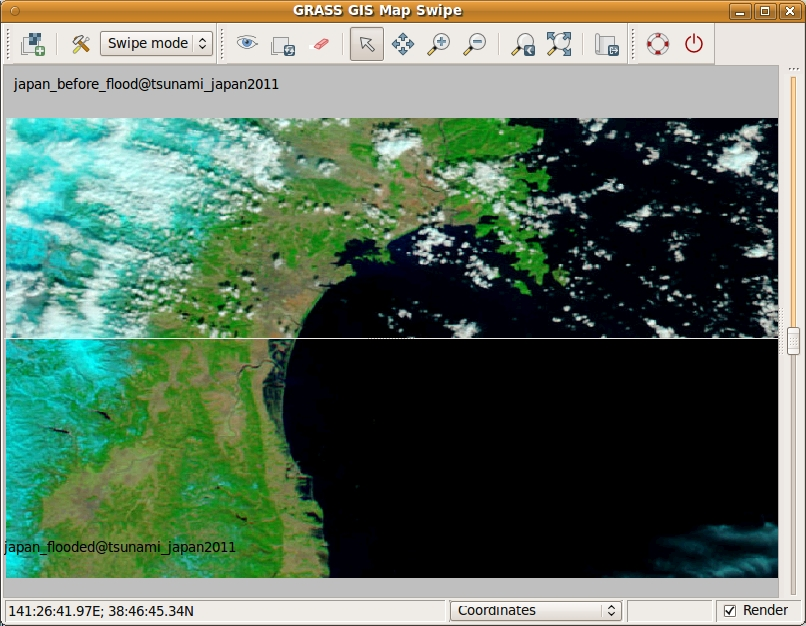
\includegraphics[width=\textwidth]{./images/mapswipe_tsunami_swipe.jpeg}
    \caption{\ms tool in `swipe' mode}
    \label{fig:mapswipe_swipe}
    \end{subfigure}
    \begin{subfigure}[ht]{0.75\textwidth}
    \centering
        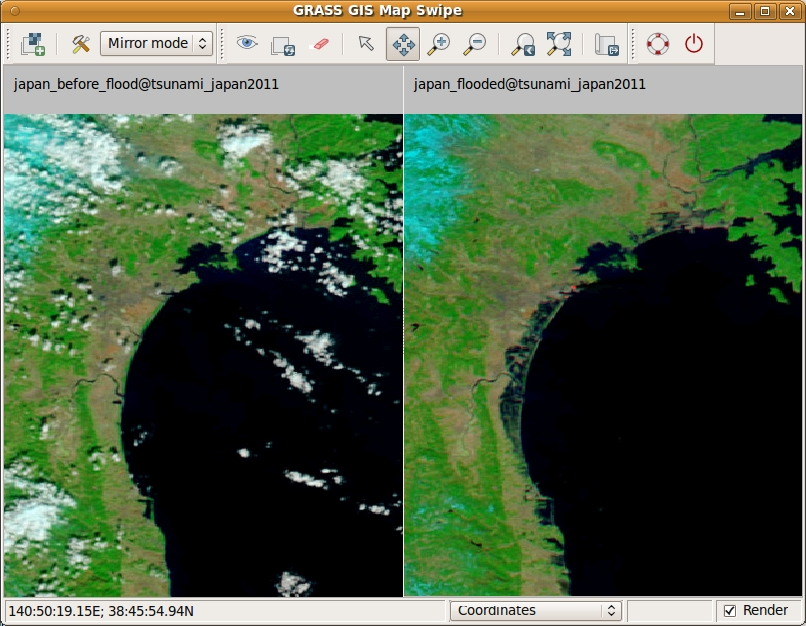
\includegraphics[width=\textwidth]{./images/mapswipe_tsunami_mirror.jpeg}
    \caption{\ms tool in `mirror' mode}
    \label{fig:mapswipe_mirror}
    \end{subfigure}
\caption[\ms tool: Pre- and post-disaster images of the tsunami in Japan in 2011]
        {\ms tool: Pre- and post-disaster images of the tsunami in Japan in 2011.
        Source: Earth Observatory/NASA}
\label{fig:mapswipe}
\end{figure}

\subsection{Features}
Map Swipe offers two different views on the raster maps.
\begin{description}
  \item[`Swipe' mode] is the default mode. It enables to compare two raster layers (of the same area)
  by revealing different parts of the maps \ref{fig:mapswipe_swipe}.
  The position of the dividing line between the two maps
  can be controlled either by dragging the line itself or dragging the slider knob which
  is located below the maps or beside them.

  \item[`Mirror' mode] enables to explore two raster maps of the same area by
  synchronizing the display region \ref{fig:mapswipe_mirror}. When a user zooms
  to any of these maps, the other one is kept synchronized.
\end{description}

These two modes can be switched dynamically. Thanks to this, GRASS users can
examine the data from different view without any other necessary steps, like loading
the maps separately into different Map Displays.

Other features include:
\begin{itemize}
    \item switching the orientation of the border line (horizontal or vertical)
    \item switching the position of the maps
    \item changing the loaded raster maps
    \item zooming, panning, zooming to map, zooming back
    \item save display to graphic file
    \item text labels with the maps' names to identify currently displayed maps
    (it is possible to move them so that they can be placed appropriately)
\end{itemize}

    
\subsection{Usage}
\ms can be launched either from Layer Manager menu (\emph{File} $\rightarrow$ \emph{Map Swipe}) or
as a module \module{g.gui.mapswipe}.
In case of launching from Layer Manager with two selected raster layers,
\ms automatically loads these layers so that the user does not have to select them again.

The advantage of the \ms as a separate module is the consistency with the GRASS design based on
separate modules. Moreover, many GRASS users prefer to use command line interface.
Therefore, \ms defines options which maps to load.
The complete interface is available by typing:

\begin{small}
\begin{lstlisting}[style=mybash]
> g.gui.mapswipe --help

Description:
 Allows to interactively compare two maps by swiping.

Usage:
 g.gui.mapswipe [first=name] [second=name] [mode=value] [--verbose]
   [--quiet]

Flags:
 --v   Verbose module output
 --q   Quiet module output

Parameters:
   first   First (top/right) raster map
  second   Second (bottom/left) raster map
    mode   View mode
           options: swipe,mirror
           default: swipe
            swipe: swiping the upper map layer
                   to show the map layer below
            mirror: synchronized maps side by side

\end{lstlisting}
\end{small}

The following example \cite{mapswipeWiki} can be run in the command line to test
the \ms tool with North Carolina sample dataset%
\footnote{download: \url{http://grass.osgeo.org/sampledata/north_carolina/nc_spm_08_grass7.tar.gz}}:
\begin{small}
\begin{lstlisting}[style=mybash]
# set computation region
g.region rast=lsat7_2002_10 -p

# create RGB composites, first color-balance:
# data from 1987
i.landsat.rgb b=lsat5_1987_10@landsat g=lsat5_1987_20@landsat \
r=lsat5_1987_30@landsat

r.composite b=lsat5_1987_10@landsat g=lsat5_1987_20@landsat \
r=lsat5_1987_30@landsat out=lsat5_1987.rgb

# data from 2002
i.landsat.rgb b=lsat7_2002_10 g=lsat7_2002_20 r=lsat7_2002_30

r.composite b=lsat7_2002_10 g=lsat7_2002_20 r=lsat7_2002_30 \
out=lsat7_2002.rgb

# .. now load the two RGB composites into the "Map Swipe" tool.
g.gui.mapswipe first=lsat5_1987.rgb second=lsat7_2002.rgb
\end{lstlisting}
\end{small}

Also, a small video tutorial is available on GRASS-Wiki page \cite{mapswipeWiki}.

\subsection{Implementation}
The essential and most problematic part of the implementation was the part responsible
for the `swiping' behavior. It was necessary to achieve smooth movement of the border line
and precise alignment of the maps. Furthermore, in order not to duplicate code providing
e.g.\ zoom functionality, it was desirable to reuse existing classes as much as possible.

The implementation consist of two main points:
    \begin{description}
      \item [Size of canvas and position of map] The tool should behave as if there was only one canvas with two map layers
      and a moving border line (one of the maps visible on each side of the border).
      To achieve such behavior I used two canvases which were placed inside a splitter widget%
      \footnote{Splitter is a common name used in GUI frameworks for a widget which manages layout of other widgets.}.
      Each canvas displays one of the two maps. To make it look like it is only one canvas,
      special `trick' is necessary. Both canvases pretend that their actual size is different from the real one%b
      \footnote{This is done by overriding a wxPython method which returns the size of a widget}.
      In case of vertical border line, we are trying to pretend
      that the width of each canvas is the sum of widths of both canvases.
      Also, the map of the right canvas must be drawn on a shifted position, so that we see the right part of it.
      
      \item [Custom mouse events] The approach described above displays the maps correctly.
      However, it introduces additional problems related to mouse events generated by mouse movement,
      clicking or dragging which are essential for zoom and pan functionality.
      This was solved by using custom mouse event class. The coordinates reported by events are shifted too,
      according to the current position of the border line. Since it is not possible to subclass mouse events,
      the right approach is to catch the original mouse event and reraise it as a custom event with changed attributes.
      This approach is used in \emph{wx.FloatCanvas} widget and has been discussed on wxPython mailing list%
      \footnote{See thread `Mix-in to base events' on wxPython-users \url{http://groups.google.com/group/wxpython-users/topics}}.
    \end{description}

Thanks to the described design, it was relatively easy to implement the `mirror' functionality.
Actually, we get the `mirror' behavior when we just simply omit the described techniques above.

\subsection{Future development}
The wiki page \cite{mapswipeWiki} of \ms lists possible enhancement of this tool
so that anybody can express his ideas. Some of this ideas were already implemented
(for example saving display to graphic file which was not in the initial prototype).

One of the most useful improvements would be to add the ability to display
more map layers, for example a combination of raster layer with vector overlay.
Unfortunately this generalization of layer management is not so simple
because it requires adding, removing and changing the order of layers.
However it would be beneficial for other wxGUI components which tackle a similar problem
(e.g.\ Supervised Classification Tool).

\section{GUI for temporal modules}
Although the \tf is fully working from command line, it is not yet introduced in the GRASS wxGUI.
This means that automatically generated GUI dialogs (refer to \ref{sec:grasswxgui})
for all temporal modules work only partially because the widget for the selection of GRASS elements
(like raster, 3D raster, vector, region, etc.) is not able to display the new temporal elements
(space time datasets). As a consequence, user has to type the name of the dataset manually
instead of selecting the available dataset from a list.

To support the selection of temporal elements in the GUI, four new elements were
added\,---\,strds (space time raster dataset), stvds (space time vector dataset),
str3d (space time 3D raster dataset) and stds (space time dataset).
Figure \ref{fig:gselect} shows the widget offering a tree view of the space time datasets
organized according to mapsets and type of dataset.
Originally, this widget supported only two levels of tree structure,
for the case of stds element one more level, the dataset type, was needed.

\begin{figure}[h!]
  \centering
  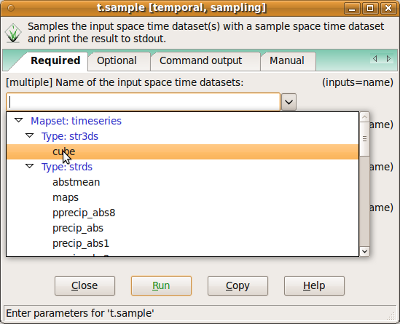
\includegraphics{./images/gselect.png}
  \caption{Element selection widget showing space time datasets}
  \label{fig:gselect}
\end{figure}

Apart from this problem, the auto-generated dialogs suffered from
not well organized module options and flags. This means that all input widgets
are together no matter what are their purposes.
Figure \ref{fig:gselect} shows two main tabs, Required and Optional,
where all options are located by default.
Since many temporal modules have no required parameters, tab Optional
contains all parameters. This can be avoided by specifying
custom `guisection' in the header of temporal module's main file
where the options and flags are described. This way, several modules
were changed by arranging the options and flags into different sections, represented
by the individual tabs (e.g.\ Input, Formatting), which makes the
GUI easier to use.

Other corrections were done to improve the appearance of the GUI. For example,
see the improvement in figure \ref{fig:forms}.
\begin{figure}[h!]
  \centering
  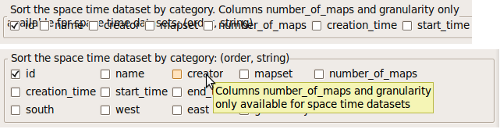
\includegraphics{./images/forms.png}
  \caption[A cutout of \module{t.list} dialog window]
  {A cutout of a dialog window of t.list module:
  the upper part shows the option appearance before and the bottom part after the correction.
  (Not all check boxes are visible in the upper part.)}
  \label{fig:forms}
\end{figure}


All these problems are related to the GUI only and the behavior of the \tf
remains untouched. 

\chapter{Conclusion}


\newpage
\clearpage
\phantomsection
\addcontentsline{toc}{chapter}{\bibname}
\printbibliography

\cleardoublepage
\phantomsection
\addcontentsline{toc}{chapter}{\listfigurename}
\listoffigures
\cleardoublepage
\phantomsection
\addcontentsline{toc}{chapter}{\listtablename}
\listoftables

\appendix
\chapter{Minard’s map of Napoleon’s 1812 campaign into Russia}
\label{appdx:minard}
\begin{singlespace}
\begin{center}
\setlength{\extrarowheight}{3pt}
 \begin{tabularx}{\linewidth}{lX}
 Author:& Charles Joseph Minard (1781 -- 1870)\\
 Title:& Figurative Map of the successive losses in men of the French Army in the Russian campaign 1812-1813.\\
 Published: & 1869 in Paris \\
 Legend:& The numbers of men present are represented by the widths of the colored zones
 at a rate of one millimeter for every ten-thousand men; they are further written across the zones.
 The red [now brown] designates the men who enter into Russia, the black those who leave it.
 The information which has served to draw up the map has been extracted from
 the works of M. M. Thiers, of Segur, of Fezensac, of Chambray, and the unpublished
 diary of Jacob, pharmacist of the army since October 28th.
 In order to better judge with the eye the diminution of the army,
 I have assumed that the troops of prince Jerome and of Marshal Davoush who had been detached
 at Minsk and Moghilev and have rejoined around Orcha and Vitebsk, had always marched with the army.\\
 Note: & 
The scale is shown on the center-right, in ``lieues communes de France'' (common French league)
which is 4,444~m (2.75~miles).
The lower portion of the graph is to be read from right to left. It shows the temperature on the army's return
from Russia, in degrees below freezing on the Réaumur scale. (Multiply Réaumur temperatures by $1 ^1\!/\!_4$ to get Celsius,
e.g. $-30\text{\textdegree} R = -37.5\,\text{\textcelsius}$).
At Smolensk, the temperature was $-21$° Réaumur on November 14th.\\
Source:& Wikipedia, The Free Encyclopedia
\end{tabularx}
\end{center}
\end{singlespace}

\begin{center}
  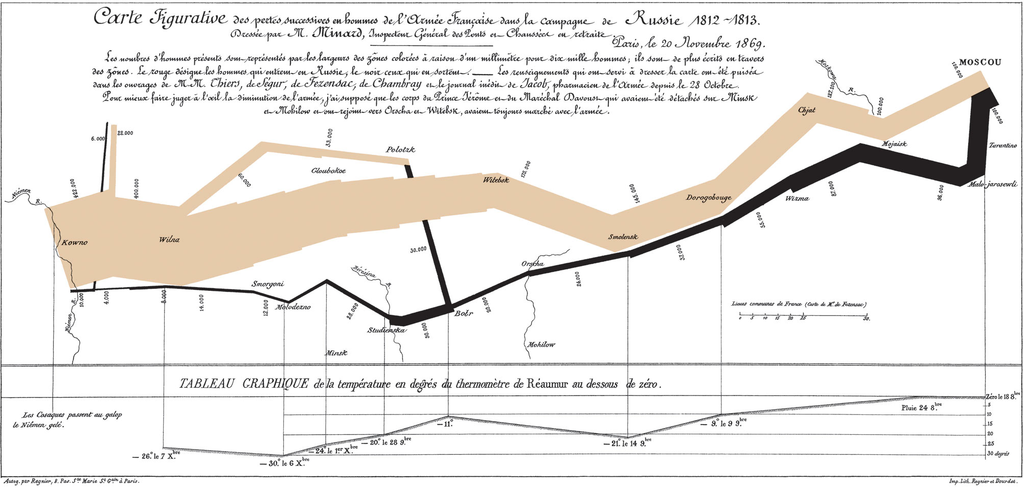
\includegraphics[width=\textheight,angle=90]{./images/Minard.png}
\end{center}


\chapter{Basic usage of the \tf library and modules}
\label{appdx:tfUsage}
The following lines illustrate a basic usage of the \tf library and modules.
Although the direct usage of the modules is more straightforward, using the library
allows to process spatio-temporal data in a more sophisticated way and to create
custom functionality not available through the modules.

\subsection*{Creating a temporal dataset using library}
The first listing demonstrates creating a new temporal dataset
and registering maps into it (as a Python script):

\begin{small}
\begin{lstlisting}[style=python]
# import temporal library and grass library
import grass.temporal as tgis
import grass.script as grass

# create a few raster maps to use them later
grass.mapcalc(exp='precip_1=rand(0,100)')
grass.mapcalc(exp='precip_2=rand(0,200)')
grass.mapcalc(exp='precip_3=rand(0,300)')
grass.mapcalc(exp='precip_4=rand(0,400)')

# initialize variables
name = 'precipitation'

# make sure the temporal database exists
tgis.init()

# create new space time raster dataset with absolute time
sd = tgis.create_space_time_dataset(
                name=name,
                type='strds', temporaltype='absolute',
                title="Title of my dataset",
                descr="Description of my dataset",
                semantic='mean')

# register these raster maps in the dataset
tgis.register_maps_in_space_time_dataset(
        type='rast', name=name,
        maps='precip_1,precip_2,precip_3,precip_4',
        start='2011-01-01', increment='3 months',
        interval=True)

\end{lstlisting}
\end{small}

\subsection*{Querying a temporal dataset using library}
The following listing shows how to query this space time raster dataset:
\begin{small}
\begin{lstlisting}[style=python]
# import temporal library and grass library
import grass.temporal as tgis
import grass.script as grass

# make sure the temporal database exists
tgis.init()

# the id of the space time raster dataset
id = "precipitation@PERMANENT"

# create the space time raster object
ds = tgis.dataset_factory(type='strds', id=id)

# check if the dataset is in the temporal database
if ds.is_in_db() == False:
    grass.fatal(_("Space time dataset <%s> not found") % id)

# select the content of the space time raster dataset object
# from the temporal database
ds.select()

# initiate helper variables to query the registered maps

# the columns that should be selected for each map
columns="id,name,mapset,start_time,end_time"

# the optional SQL where statement: select all maps with
# a start time later then 1 May 2011
where="start_time > '2011-05-01'"

# we order the rows by start time
order="start_time"

# the query
rows = ds.get_registered_maps(
        columns=columns, where=where, order=order)

# check if we found any maps
if not rows:
    grass.fatal(_("Space time dataset <%s> is empty") % id)

# simply print the map id, name, mapset and the time stamp.
for row in rows:
    print row["id"]
    print row["name"]
    print row["mapset"]
    print row["start_time"]
    print row["end_time"]

# the output
precip_3@PERMANENT
precip_3
PERMANENT
2011-07-01 00:00:00
2011-10-01 00:00:00
precip_4@PERMANENT
precip_4
PERMANENT
2011-10-01 00:00:00
2012-01-01 00:00:00

\end{lstlisting}
\end{small}

\subsection*{Creating a temporal dataset and its querying using modules}
The same functionality is available through temporal modules
which usually only wrap the library functions.
The following listing shows how to perform the same tasks as in the previous
listing by using temporal modules (in Bash command line):
\begin{small}
\begin{lstlisting}[style=python]
# we suppose maps are already created

# create new space time raster dataset with absolute time
t.create output=precipitation semantictype=mean \
title="Title of my dataset" \
description="Description of my dataset"

# register raster maps in the dataset
t.register -i input=precipitation \
maps=precip_1,precip_2,precip_3,precip_4 \
start="2011-01-01" increment="3 months"

# query temporal dataset
t.rast.list input=precipitation \
columns=id,name,mapset,start_time,end_time \
where="start_time > '2011-05-01'"

# output (changed formatting here to fit page)
precip_3@PERMANENT precip_3  PERMANENT
2011-07-01 00:00:00 2011-10-01 00:00:00
precip_4@PERMANENT precip_4  PERMANENT
2011-10-01 00:00:00 2012-01-01 00:00:00

\end{lstlisting}
\end{small}

\chapter{\at screenshots}
\label{appdx:animation}
\begin{figure}[h!]
  \centering
  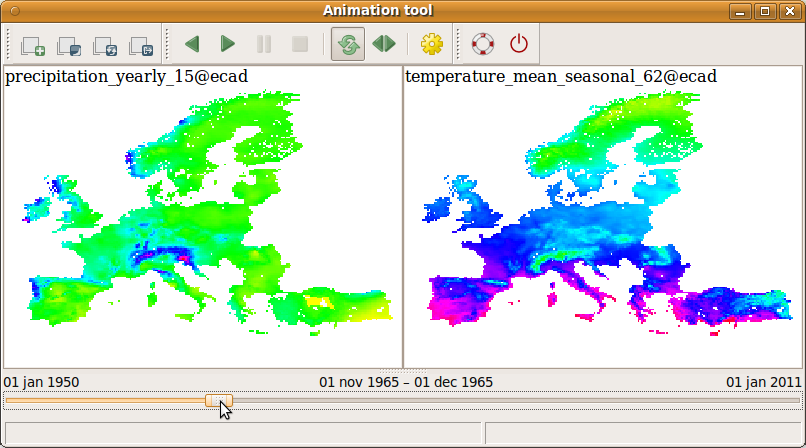
\includegraphics[width=\textwidth]{./images/animation_tool1.png}
  \caption{\at: two animations of temporal datasets with different time resolution (yearly and seasonal).
  Data source: E-OBS gridded dataset \cite{haylock2008european}.}
  \label{fig:anim2D}
\end{figure}
% We acknowledge the E-OBS dataset from the EU-FP6 project ENSEMBLES (http://ensembles-eu.metoffice.com) and the data providers in the ECA&D project (http://www.ecad.eu)


\begin{figure}[h!]
  \centering
  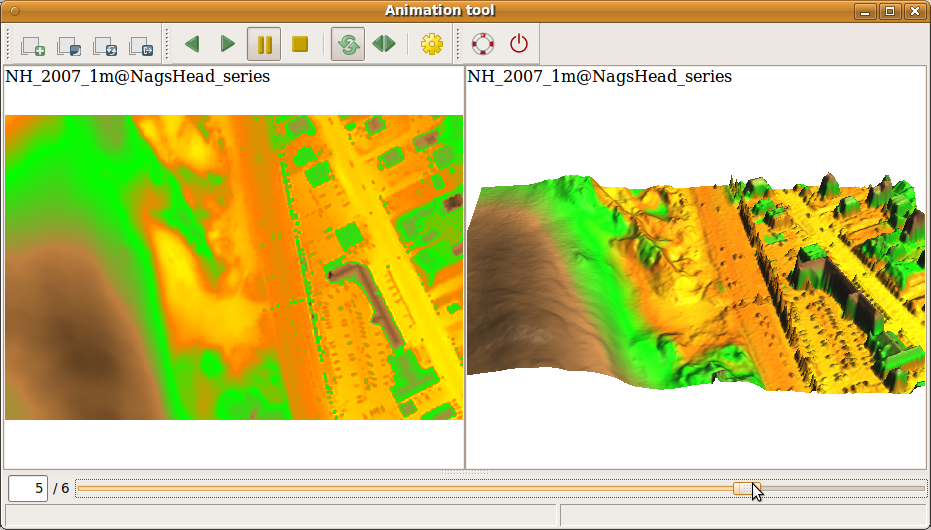
\includegraphics[width=\textwidth]{./images/animation_tool2.png}
  \caption{\at: synchronized 2D and 2.5D animation of the same area using
  multiple maps without time information. Data source: NagsHead mapset available from
  \url{http://courses.ncsu.edu/mea582/common/media/01/NagsHead_series.zip}}
  \label{fig:anim3D}
\end{figure}

\begin{figure}[h!]
  \centering
  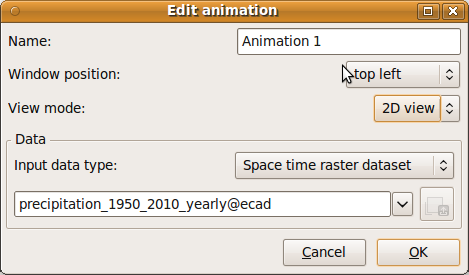
\includegraphics{./images/animation_tool_edit.png}
  \caption{\at: dialog for defining animation properties}
  \label{fig:anim_edit}
\end{figure}

\begin{figure}[h!]
  \centering
  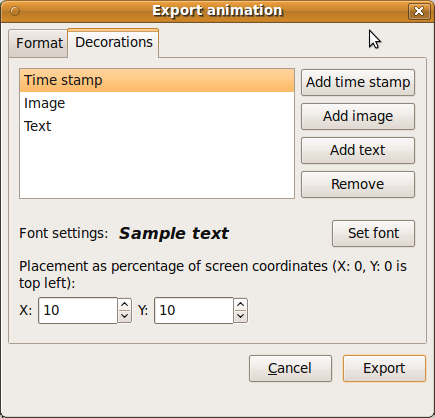
\includegraphics{./images/animation_tool_export.png}
  \caption{\at: dialog for exporting animation\,---\,adding decorations}
  \label{fig:anim_export}
\end{figure}

\begin{figure}[h!]
  \centering
  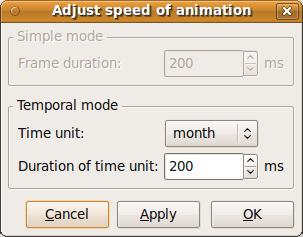
\includegraphics{./images/animation_tool_speed.png}
  \caption{\at: dialog for adjusting speed of animation (temporal mode active)}
  \label{fig:anim_speed}
\end{figure}

\end{document}
